%\documentclass[10pt,conference]{IEEEtran}
%\documentclass[9pt,conference]{sig-alternate}
%\documentclass[9pt,conference]{sig-alternate}
%\documentclass[10pt,print,letterpaper,nocopyrightspace]{sigplan-proc-varsize}
\documentclass[10pt,print,letterpaper]{sigplan-proc-varsize}

\usepackage{amsmath,epsfig}
\usepackage{url}
\usepackage{xspace}
\usepackage{colortbl}
\usepackage{subfigure}
\usepackage{dsfont}
\usepackage{boxedminipage}
\ifx\pdfoutput\undefined
\usepackage[hypertex]{hyperref}
\else
\usepackage[pdftex,hypertexnames=false]{hyperref}
\fi

\usepackage{amssymb}
\usepackage{wasysym}
\usepackage[left=2.54cm,top=2.54cm,right=2.54cm,bottom=2.54cm,nohead,nofoot]{geometry}



\DeclareMathOperator*{\argmax}{argmax}
%\usepackage{times}

\def\ucb{$^{\dagger}$}
\def\stanford{$^{\ddagger}$}
\def\arch{$^{\star}$}

\newcommand{\kb}{kB}
\newcommand{\rene}{Ren{\'e}\xspace}
\newcommand{\reneii}{Ren{\'e}2\xspace}
\newcommand{\wec}{WeC\xspace}
\newcommand{\mica}{Mica\xspace}
\newcommand{\micaii}{Mica2\xspace}
\newcommand{\micaz}{MicaZ\xspace}
\newcommand{\micadot}{Mica2Dot\xspace}
\newcommand{\iic}{I$^2$C\xspace}
\newcommand{\uA}{$\mu$A\xspace}
\newcommand{\dotmote}{Dot\xspace}
\newcommand{\mhz}{MHz\xspace}
\newcommand{\ghz}{GHz\xspace}
\newcommand{\kbps}{kbps\xspace}
\newcommand{\dsn}{DSN\xspace}
\newcommand{\io}{I/O\xspace}
\newcommand{\telos}{Telos\xspace}

\newcommand{\T}{\mathds{T}}
\newcommand{\XXXnote}[1]{{\bf\color{red} XXX: #1}}


\begin{document}

%\conferenceinfo{Sensys'08,} {November 5--7, 2008, Raleigh, NC, USA.}  
%\CopyrightYear{2008} 
%\crdata{978-1-60558-096-8/08/09} 

%\title{PEAS: The Personalized Energy Attribution System}
\title{Towards an Energy Lens on the \\Physical World with Mobile Phones}
%\numberofauthors{1} 
%\author{\alignauthor Stephen Dawson-Haggerty, Jorge Ortiz, Xiaofan Jiang and David Culler\\
%\affaddr{Computer Science Division}\\
%\affaddr{University of California, Berkeley} \\ 
%\affaddr{Berkeley, California 94720} \\
%\email{\{stevedh,jortiz,xjiang,culler\}@cs.berkeley.edu}
%} 


%\subtitle{Paper \# Insert Reg Number Here}

%\title{Alternate {\ttlit ACM} SIG Proceedings Paper in LaTeX
%Format\titlenote{(Produces the permission block, and
%copyright information). For use with
%SIG-ALTERNATE.CLS. Supported by ACM.}}
%\subtitle{[Extended Abstract]
%\titlenote{A full version of this paper is available as
%\textit{Author's Guide to Preparing ACM SIG Proceedings Using
%\LaTeX$2_\epsilon$\ and BibTeX} at
%\texttt{www.acm.org/eaddress.htm}}}
%
% You need the command \numberofauthors to handle the 'placement
% and alignment' of the authors beneath the title.
%
% For aesthetic reasons, we recommend 'three authors at a time'
% i.e. three 'name/affiliation blocks' be placed beneath the title.
%
% NOTE: You are NOT restricted in how many 'rows' of
% "name/affiliations" may appear. We just ask that you restrict
% the number of 'columns' to three.
%
% Because of the available 'opening page real-estate'
% we ask you to refrain from putting more than six authors
% (two rows with three columns) beneath the article title.
% More than six makes the first-page appear very cluttered indeed.
%
% Use the \alignauthor commands to handle the names
% and affiliations for an 'aesthetic maximum' of six authors.
% Add names, affiliations, addresses for
% the seventh etc. author(s) as the argument for the
% \additionalauthors command.
% These 'additional authors' will be output/set for you
% without further effort on your part as the last section in
% the body of your article BEFORE References or any Appendices.

\numberofauthors{2} %  in this sample file, there are a *total*
% of EIGHT authors. SIX appear on the 'first-page' (for formatting
% reasons) and the remaining two appear in the \additionalauthors section.
%
\author{
Jorge Ortiz\\
       %\affaddr{Department}\\
	\affaddr{Computer Science Division}\\
       \affaddr{University of California, Berkeley}\\
       %\affaddr{City, State Zip}\\
       \email{jortiz@cs.berkeley.edu}
}


\maketitle

%\date{14 April 2007}
%\maketitle

\begin{abstract}
Despite the growing impact of climate change and energy prices, 
per-capita energy consumption is rising. Part of the problem is visibility. We do not 
have scalable means of observing our energy consumption patterns and determining how to optimize and reduce our
consumption.
Mobile smartphones present a unique opportunity to enable an energy view on the physical world. 
They can bridge the physical world, information infrastructure, and people
through a rich set of sensors, ubiquitous connectivity, and highly personal user interface. 
With QR codes as cheap tags on items and places in the physical world, the
camera becomes a portable scanner in your pocket, in addition to its
traditional functions.  We explore this
unique triple point
and re-examine classical problems of context and consistency management in mobile
systems.  We also examine this combination as it pertains to energy management of physical
devices.  In doing so, we are re-introduced to problems of apportionment and aggregation of sensor data,
except with a continuously changing set of constituents.  We describe our solution in a technique
called \emph{dynamic aggregation} that maintains moving aggregates as the
set of data sources changes over time.  We deployed our system in a 
141,000 square-foot building, tagging 351 items over 139 room across 7 floors.

% When combined with QR codes, the on-board camera provides us with a portable scanner

% The camera,
% when combined with QR codes, gives us a portable scanner and convenient mechanism for tying these world together. 
% In this paper, we describe our system and deployment experience for a mobile phone application the provides 
% user-centric energy-view of the physical world. We describe the challenges, specifically dealing with mobility, 
% and how we address them in a set of three separate applications: an energy auditing application, a 
% device energy scanner, and a personal energy counter. We also introduce a technique called \emph{dynamic aggregation}
% which allows us to seamlessly track the constituents of aggregated energy calculations, as they move from one 
% location to another.

% Despite the recent impact of global warming and a steady increase in energy prices, 
% per-capita energy consumption is rising. Part of the problem is about visibility. We simply do not 
% have any good ways of seeing how we consume energy, and therefore, how to optimize and reduce it. 
\end{abstract}

% A category with the (minimum) three required fields
%\category{B.0}{Hardware}{General}
%\category{B.4}{Hardware}{Input/Output \& Data Communication}

%\terms{Design, Implementation, Performance, Experimentation}

%\keywords{Churn, Link, Routing, Wireless, Sensor Network, Mote}

%\newpage

\subsection{Introduction}
The United States leads the world in per-capita energy consumption.
Our electricity use has consistently increased over the last 40 years~\cite{oecd2011} and other parts of the world are rising all 
too rapidly.  With the specter of climate change and the increasing cost of energy, we must explore new
ways for individuals to gain visibility and insight into their energy consumption in order to optimize and reduce it. 
With the increasing penetration of embedded sensors in the environment and
the continued rise in smartphone adoption, we see an opportunity for smartphones to bridge the physical world
to our computational infrastructure and provide an `energy lens' on the physical world.  

We use mobile phones to construct an entity-relationship 
graph of the physical world and combine it with streaming sensor data in order to perform detailed energy-attribution.
We limit the scope of the world to a single building domain.  We have designed and implemented a real-time, mobile energy auditing
application, called the `Energy Lens', that allows us to collect information about 
things throughout the building and how they are related to each other.  For example, computer X is inside 
room Y and connected to meter Z.  Then, we use these relationships to guide our data look-up and analytical
calculations.  For example, the load curve of room Y consists of the sum of all the power traces for loads
inside room Y.  We use the mobile smartphone as the main input tool.  Our work examines \emph{three main challenges} in setting up and 
deploying a real, whole-building infrastructure to support real-time, 
fined grained energy analytics.  

The first challenge is related to tracking and mobility.
The use of mobile phones presents classical, fundamental challenges related to mobility.  Typically, mobility
refers to the phone, as the person carrying it moves from place to place.  However, in the energy-attribution
context, we are also referring to the movement of energy-consuming objects.  Tracking their relationships to spaces 
and people is as important as tracking people.  We describe how we deal with \emph{both moving people and 
moving objects} and show that these historically difficult problems can be addressed relatively easily, if the proper infrastructure is 
in place.  %We provide evidence that the approach is simple, incrementally deployable, and scalable.

The second challenge is about capturing the inter-relationship semantics and having these inform our  analytics.
We adopt the general notion of physical tags that identify objects in the world.  Our system uses \emph{QR codes} to tag things and locations 
in the physical world.  However, \emph{any tag that provides a unqiue identifier for an object could serve the same purpose}.
Once tagged, there are three types of interactions -- 
registration, linking, and scanning -- which establish important relationships.  Registration is the act of creating a virtual object 
to represent a physical one.  Linking captures the relationship between pairs of objects.  Scanning is the act of performing an item-lookup.
Each of these interactions requires a set of swiping gestures.  Linking requires two tag swipes while the other two actions
require a single tag swipe.  Internally, we maintain a \emph{entity-relationship graph (ERG)} of things, people, and locations, that gets
updated through these sets of gestures.

The third challenge is about indoor network connectivity and access.
In order to connect these components, we rely on having `ubiquitous' network connectivity.  However, in practice, network
\emph{availability} is intermittent and our system must deal with the challenges of intermittency.  We discuss how caching
and logging are used to address these challenges.  Moreover, when connectivity is re-established, we must deal with
applying updates to the ERG, as captured by the phone while disconnected.  
% Conflicts can also occur during an update.  For example, the two updates may disagree about which items are attached
% to which meters.  We implement a very simple conflict resolution scheme, described in section~\ref{sec:conflicts}.
% Finally, certain physical-state transitions are represented as a set of updates to the ERG that must be applied 
% atomically.  We implement transactions in the log-replay and transaction manager.
% Our `Energy Lens' system is deployed in a building on our campus.  We discuss
% its architecture and our design choices.  
  
% We also discuss novel strategies for tracking moving people/things and describe how we implement these in our system.  In summary, our work
% makes the following contributions:

% \begin{itemize}
% \item We design and implement a system that captures and combines physical entities, their inter-relationships, and real-time sensor data 
% 		in buildings.% using mobile phones, qr code, and a cloud-based infrastructure.
% \item We observe that certain combinations of swipes give us useful information to set the location of people and things over time.
% 		We codify this observation in our \emph{context-tracker} and use it to maintain consistency between the entity-relationship graph and the 
% 		state of the physical world.  To the best of our knowledge, this is radically different from the approaches in standard 
% 		localization techniques.  However, we argue that it can be used to \emph{enhance} their accuracy and overall performance.
% \item We implement a prefetching algorithm to obtain context-dependent information to both improve performance and
% 		enable disconnected operation.  We also design and implement a log-replay and transaction manager over our data management layer.  We describe how different conflict-resolution policies can be implemented and our rationale for the policies we chose.
% \end{itemize}

% \vspace{0.08in}

% In the next sections we go through a motivating scenario.  We then discuss some related work, followed 
% by the system architecture, evaluation, and future directions.

\section{Related work}

%\begin{itemize}
% \item dashboard
% \item andrew's lightin control work
% \item Kamin's hvac control work
% \item BEMs
% \item sMAP stuff
%\item Buildsys 2010 work~\cite{hbci}
%\item distributed consistency management: COPS
%\item mobility: tracking things with RFID~\cite{rfid_gonz2006}
%\item mobility: tracking of people, wifi indoor localization
%\item entity-relationship graphs
%\item homeOS [microsoft]
%\item HP Cooltown~\cite{cooltown}
%\end{itemize}
Our work touches on several areas from smart home research to logistics.  In the building space, there has been
some interest in building various kinds of energy-related visual and control applications.
This work focuses on the object definition, tracking, and management component of the architecture proposed by 
Hsu et al.~\cite{hbci}.  Their work stratefied the set of challenges that one could potentially face if the application 
were deployed at scale.  Our
work, in constrast, bases its design rationale on a \emph{real deployment} that is taking place at scale in a building 
on our campus.  We focus on solving fundamental systems challenges in dealing with intermittent connectivity
and conflict resolution in tracking people and things over time.  We also focus on leveraging gestures to minimize
the cost of interaction for users, while maximizing the information we can attain about the state of the world.

% Tracking people/indoor localization
An important aspect of the Energy Lens is determining when people and things have moved.  This requires some form 
of indoor localization.  There's a large body of literature in the area of indoor localization with mobile phones ranging from 
using wifi~\cite{radar}, to sonar~\cite{cricket}, to ambient noise~\cite{abs}, and a combination of sensors on the 
phone~\cite{surroundsense, darwinphone}.  Dita~\cite{dita} uses acoustic localization of mobile phones and also uses the infrastructure 
to determine gestures in free-space that are classified into pre-defined control actions.  Each of these require relatively complex 
software and/or infrastrure.  
We take a radically different, simple approach.  We use cheap, easy to re/produce tags (QR codes), place them on things in the 
environment over incrementally and use the natural \emph{swiping gesture} that users make, when interacting with the Energy Lens 
application, to track when they have moved or when the objects around them have moved.  The working principal is to attain as much 
information from their gesture to determine when something/one has moved.  We discuss our heuristics in section~\ref{sec:swipes}.

% context-aware apps
ACE~\cite{ACE} uses various sensors on the phone to infer a user's context.  The context domain consists of a set of user activities
and semantic locations.  For example, if ACE can distinguish between {\tt Running, Driving, AtHome, or InOffice}.  ACE also infers 
the one from the others, so if the user is {\tt AtHome} then they are not {\tt InOffice}.  Energy Lens uses inference to determine
when a person or thing has moved.  Certain swipe combinations give us information about whether they moved and where they moved to or
whether an item moved and where it moved to.  The main difference is that we only infer context when a user is actively swiping, rather
than a continuous approach.  Pretching is a fundamental technique used in many domains.  However, the cost of a prefetch for mobile
application outways the benefits if the prefetched data is not useful.  Informed mobile pretching~\cite{IMP} uses cost-benefit analysis 
to determine when to prefetch content for the user.  In the Energy Lens context, we prefetch data based on their location swipes.
We also rely on pretching to anticipate loss of connectivity, not just to improve preformance.

% Tracking things
Logistic systems focus on the tracking of objects as the move through distribution sites to warehouses, stores, shelves,
and purchase.  Items are tracked through bar code or RFID readers.  However, the workload is very structured and well
defined.  The authors of~\cite{rfid_gonz2006} describe this structure and leverage it to minimize storage
requirements and optimize query-processing performance.  Energy Lens uses the QR codes as the tag and the phone as an active
reader.  As objects move, users scan those items to their new location.  However, objects may belong to one or
many people, they can be metered by multiple meters a day, and their history in the system
is on-going.  In contrast, a typical logistics workload has a start (distribution site) and end point (leaving the store
after a sale).  In our workload, relationship semantics are important; we need to know whether the meter is \emph{bound-to}
rather than simple \emph{attached-to} an item.  We discuss the difference later in the paper.
% In addition to traditional logistics-style queries -- \emph{What is the average time that it took coffee-makers to move from the 
% warehouse to the shelf and finally to the checkout counter in January of 2004?} -- energy-analytics requires queries to group
% partial traces from meter data by tracking what meters the item attached to over the specified time-frame.
% The Energy Lens system collects and manages this kind of information to enable such queries.
Furthermore, we take advatange of natural gestures the user makes with the phone while scanning QR codes to extract
information about the current location of the user or things.

% Tagging items, virtual services
The key idea in the HP Cooltown~\cite{bridgingphysical,cooltown} work is to web-enable `things' in the world, grouped-by
`place', and accessed by `people' via a standardized acquisition protocol (HTTP) and format (HTML, XML).  
Cooltown creates a web presence for things in the world either directly (embedded web server) or indirectly 
(URL-lookup tag) as a web page page that display the services it provides.  Many of the core concepts in Cooltown 
also show up in Energy Lens.  The main overlap is the use of tags in the world that contain a reference to a virtual 
resource, accessible via HTTP through
a network connection.  Cooltown, however, explicitly chooses not maintain a centralized relationship
graph, it leverages the decentralized, linking structure of the web to group associated web pages together.
Furthermore, things are assumed to not move.  People are the main mobile entities.  The kind of applications
we wish to support must track where things are and their specific inter-relationships.  We imposed a richer set of 
semantics on our, centrally maintained, relationship graph and use it to provide detailed energy information.


\section{System Architecture}
Our architecture consists of three components: mobile phones, QR codes, and a web application stack sitting in
the cloud.  The goal of our architecture is to enable virtual services on the physical world and to use the mobile
phone as an intrinsic element of those services.  An instance of our architecture was deployed inside a building and we make the
following assumptions for our archicture to deliver our goals successfully:

\begin{enumerate}
\item Most building occupants own a smartphone that they carry with them most of the time.
\item Network connectivity is available throughout the building.
\end{enumerate}
\vspace{0.06in}

Figure~\ref{fig:sysarch} shows an overview of the components of our archiecture.  We place QR codes on items throughout
the entire building.  This includes all building entrances, floors, rooms, and energy-consuming devices.  Occupants
use their phone and personal printer to add new items.  For items that are already registered, occupants use their phone
to scan their tags to learn more information about the items and to participate in maintaining a consistent
view of the building.  We discuss each of the three components in further detail in the following sections.

% Our architecture consists of various components, with the mobile phone serving as the centerpiece.  Smart phones
% serves as a point of intersection between the user, her environment, and compontational infrastructure.  Smarts phones
% are highly personalized, are carried by users everywhere, and with ubquitous, multi-modal forms of accessing a network,
% provide almost continuous access to services.  However, although space and context are nebulous ideas and difficult to capture
% we can learn from user feedback.  In order to truly bridge the physical world to the virtual world, we include the use
% of QR codes to tag \emph{any item the user finds relevant to capture}.  QR codes are easy to generate and inexpensive
% to produce and replace.

% With energy tracking as the main goal, we used QR codes to tag items that consume energy.  When an item is tagged, the user swipes
% the tag and enters information about the item.  After this `registration phase' is complete, any user can use
% their smart phone to learn about the item by swiping the QR code that is attached to it.  In addition to arbitrary
% descriptive metadata, we distinguish between regular items and \emph{meters}.  Meters are items that produce
% continuous energy data.  Meters are bound to items that are attached to them and serve as a proxy for the energy information
% about the device it is attached to.  We describe how \emph{binding} between items is done in section~\ref{sec:binding}.
% Figure~\ref{fig:sysarch} shows our system architecture and each of the components.

%FILL IN WITH REAL GRAPH
\begin{figure*}[htb!]
\begin{center}
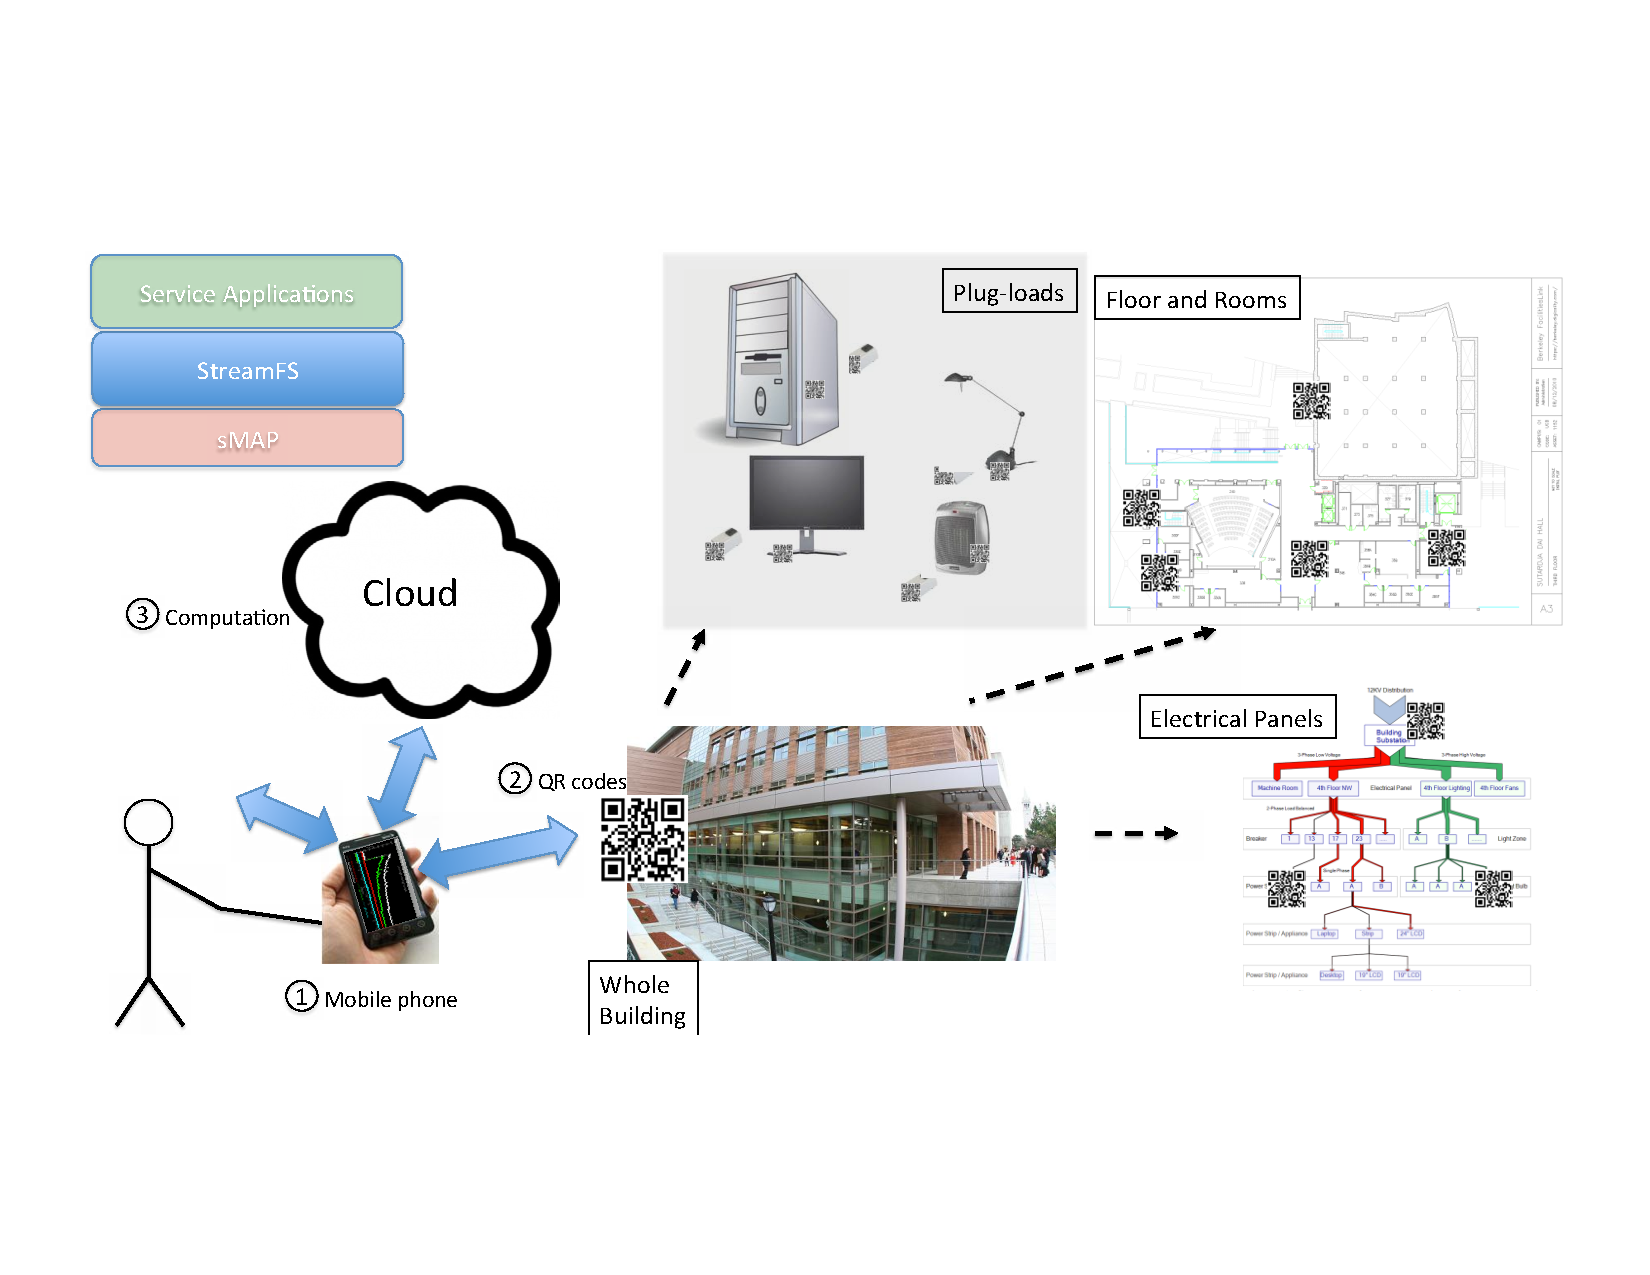
\includegraphics[width=0.8\textwidth]{figs/sysarch}
\caption{Above we show the system architecture.  The main components are mobile phone, QR codes, and access to cloud
our services.  The mobile phone serves as the triple-point of the architecture: it serves as the point of
intersection between the human, the physical world, and cloud services. }
\label{fig:sysarch}
\end{center}
\end{figure*}

\subsection{Mobile phone}
\label{sec:mobilephone}
% The mobile phone is at the center of our architecture.  Its basic function is to swipe QR codes in the environment,
% do a lookup to the backend through the network, query for any relevant information to display to the user and display it.
% Interaction with the user is through this set of displays.  For example, if a user wish to learn more about when
% their television was on, they swipe the QR code on the television.  The phone offers various services that the television
% provides.  In the current set of application we have written, you would get to read the description, make, and model of the
% television.  You might also learn what the rated power of the television, if that was included in the metadata capture.
% If the television has a meter attached and that meter is virtually and physically bound to it, on of our applications
% also allows you to view the power traces associated with television over various time intervals.  The default is 24-hours.

The mobile phone is the main component of our architecture.  It is a unique triple-point: the point of intersection
between people, physical objects, and computational infrastructure.  We take advantage of the engineering that has gone 
into making the interaction between the phone and its owner quite natural in order to give us personal and contextual
information.  For example, users naturally point towards items they are interested in capturing (when a picture is taken).
We use this gesture to capture physical objects and incorporate them in our virtual representation of the world.
People use their mobile phone camera to scan QR codes in the environment.  This can be used to obtain information
about where they are, to obtain information about the object, or to obtain information about the relationship
between objects. A simple gesture can provide the individual with a 'user
inerface' for the room and the devices within it.
\cite{Enabling ``Smart Spaces:'' Entity Description and User Interface Generation for a Heterogeneous Component-based Distributed System 
T. D. Hodes, R. H. Katz, DARPA/NIST Smart Spaces Workshop, 
Gaithersburg, Maryland, July 1998. 
UC Berkeley Technical Report CSD/98/1008}
The screen can be used as a secondary input/output to give us/them more information about the 
object or context.  We discuss these in more details in Section~\ref{sec:apps}.

\subsection{QR Codes}
\label{sec:qrc}

A QR code is a two-dimensional barcode that may encode almost 3000 bytes of data.  QR code generators
can be found on the internet~\cite{qrcgen1, qrcgen2}.  
Extending the approach in \cite{hbci}, in
our
architecture the QR code contains a meaningful {\tt URL} that a
generic browser can access to provid ea human readable document with complete
information about the item or space, as well as the additional
information to bootstrap the smartphone to optimized access, such as
native apps for interacting with the item or space.  Secondly, the 
{\tt URL}  must be easily transformed into one that will yield a
programmatic document, such as a JSON object, that apps can
manipulate.  And finally, the representation of the URL itself can be
parsed and utilized locally by native apps, typically by lookup, to
permit rapid interaction with the item or space.

\begin{figure}[htb!]
\begin{center}

\includegraphics[scale=0.3]{figs/qrcex}
\caption{This is an example QR code from our deployment. This label resolves to {\tt http://tinyurl.com/6235eyw}.
QR codes like these are used as tags physical objects and spaces/locations.}
\label{fig:qrcex}
\end{center}
\end{figure}

Figure~\ref{fig:qrcex} shows an example QR code used in our deployment.  Tags like these are placed on physical
objects and spaces throughout the building to link between the physical world and our virtual representation of it.
QR codes are cheap to produce.  Any printer and some tape can be used to tag an item.  This is important for scalability.
With the number of physical objects and places (floors, rooms) in a typical building, {\bf we must rely on the occupants
to scale our deployment}. Because QR codes are easy to produce, we can provide occupants with a webpage that
that produces them.  They print them out, place them on items or
places they want to interact with, register them, and provide useful
information about them.

Generating the right kind of QR code is important.  It is trivial to
encode information onto them, but it is
not trivial to design them so that they encode just enough information to be useful.  If 
too much information is encode the camera takes a long time to scan them, especially under poor lighting
conditions.  This can easily frustrate and drive away users, who are critical for scalability.
We also want to design them for the lowest common denominator in terms of camera quality.  Older
phones with cheap cameras should also be able to scan the tags quickly.  We ran some experiments to show
how complex QR codes differ from the one we design and discuss these results in Section~\ref{sec:qrcodedesign}.


\subsection{Computational infrastructure}
% The third piece of our architecture consists of a data collection and management components.  The subcomponents
% of this part of the archictecture are set up in layered fashion.  The context and data mangement layer is at the top,
% the meter-access layer is below that, and at the bottom is the metering infrastructure.  The context layer sets up
% a structured metadata organization whose semantics are interpretted by each application.  We describe the single structure
% that supports our applications.  In addition, this layer unifies the metadata and the data, allowing the application
% to access all meters data that share similar properties (i.e. placement, type, owner, etc.).  The meter data-access layer 
% unifies the various access standards into a single interface.  This allows us to add sensors and easily incorporate it
% into our context layer.  Finally, we integrated various types of meter data.  Specifically, we used several wireless
% power meters called ACmes~\cite{acme} as well as various streams from the building management system directly.

The final piece of our architecture consists of three layered
components for meter and usage data representation,
data and metadata managament, and applications.  Each layer in the stack is network accessible and hosted on a combination
of machines we own and across two cloud-service providers.  The distributed nature is a testament to the flexibility of
placement for each of the pieces.  However, the layering is imposed in our setup.  Physical data streams,
coming from wireless power meters~\cite{acme}, weather feeds from weather underground~\cite{weatherunderground}, the
local building management system are directed towards the sMAP~\cite{smap}, above these feeds then forward their data
to our context management layer, StreamFS~\cite{streamfs}, and finally, we build our applications on top of StreamFS.
We describe each of these in the following sections.

\subsubsection{Application layer}
At the application layer we use a standard Apache web server~\cite{apache}.  Two of our apps -- the item
energy scanner and the personal energy counter -- are essentially just web applications.  When the phone scans a tag, it
re-directs to the main page which shows a list of services for that item that was scanned.  It also provides an option
to the user to login in to obtain a peronalized energy view.  We discuss the details of these applications as well
as the energy auditing application, which is a native app, in Section~\ref{sec:apps}.

\subsubsection{sMAP}
\label{sec:smap}
%Disucss how the streaming meter data is forwarded to streamfs and linked to streamfs objects.
sMAP~\cite{smap} provides a uniform data access layer for sensor information.  We can take any of the various sensor protocols
and make it accessible through sMAP's HTTP, RESTful API.  In addition, sMAP servers can live on any machine that is accessible
through the web.  This is convenient for our purposes, since it makes the raw sensor data stream accessible through any network.
sMAP's data-forwarding facility is used extensively to link the sensor data with the context layer.  When a meter is being added
to the context layer, a callback is installed on the sMAP server that hosts that meter's stream.  As meter data is reported 
to the sMAP server, it is forwarded to the appropriate node {\tt URL} in StreamFS, setting up the context associated with that
meter automatically.

% \subsection{Metering layer}
% We used several types of meter data in our applications.  Specifically we integrated the whole-building building power-draw feed,
% and a number of feeds from our wireless ACme power-meter deployment.

%FILL IN WITH REAL GRAPH
\begin{figure*}[htb!]
\begin{center}
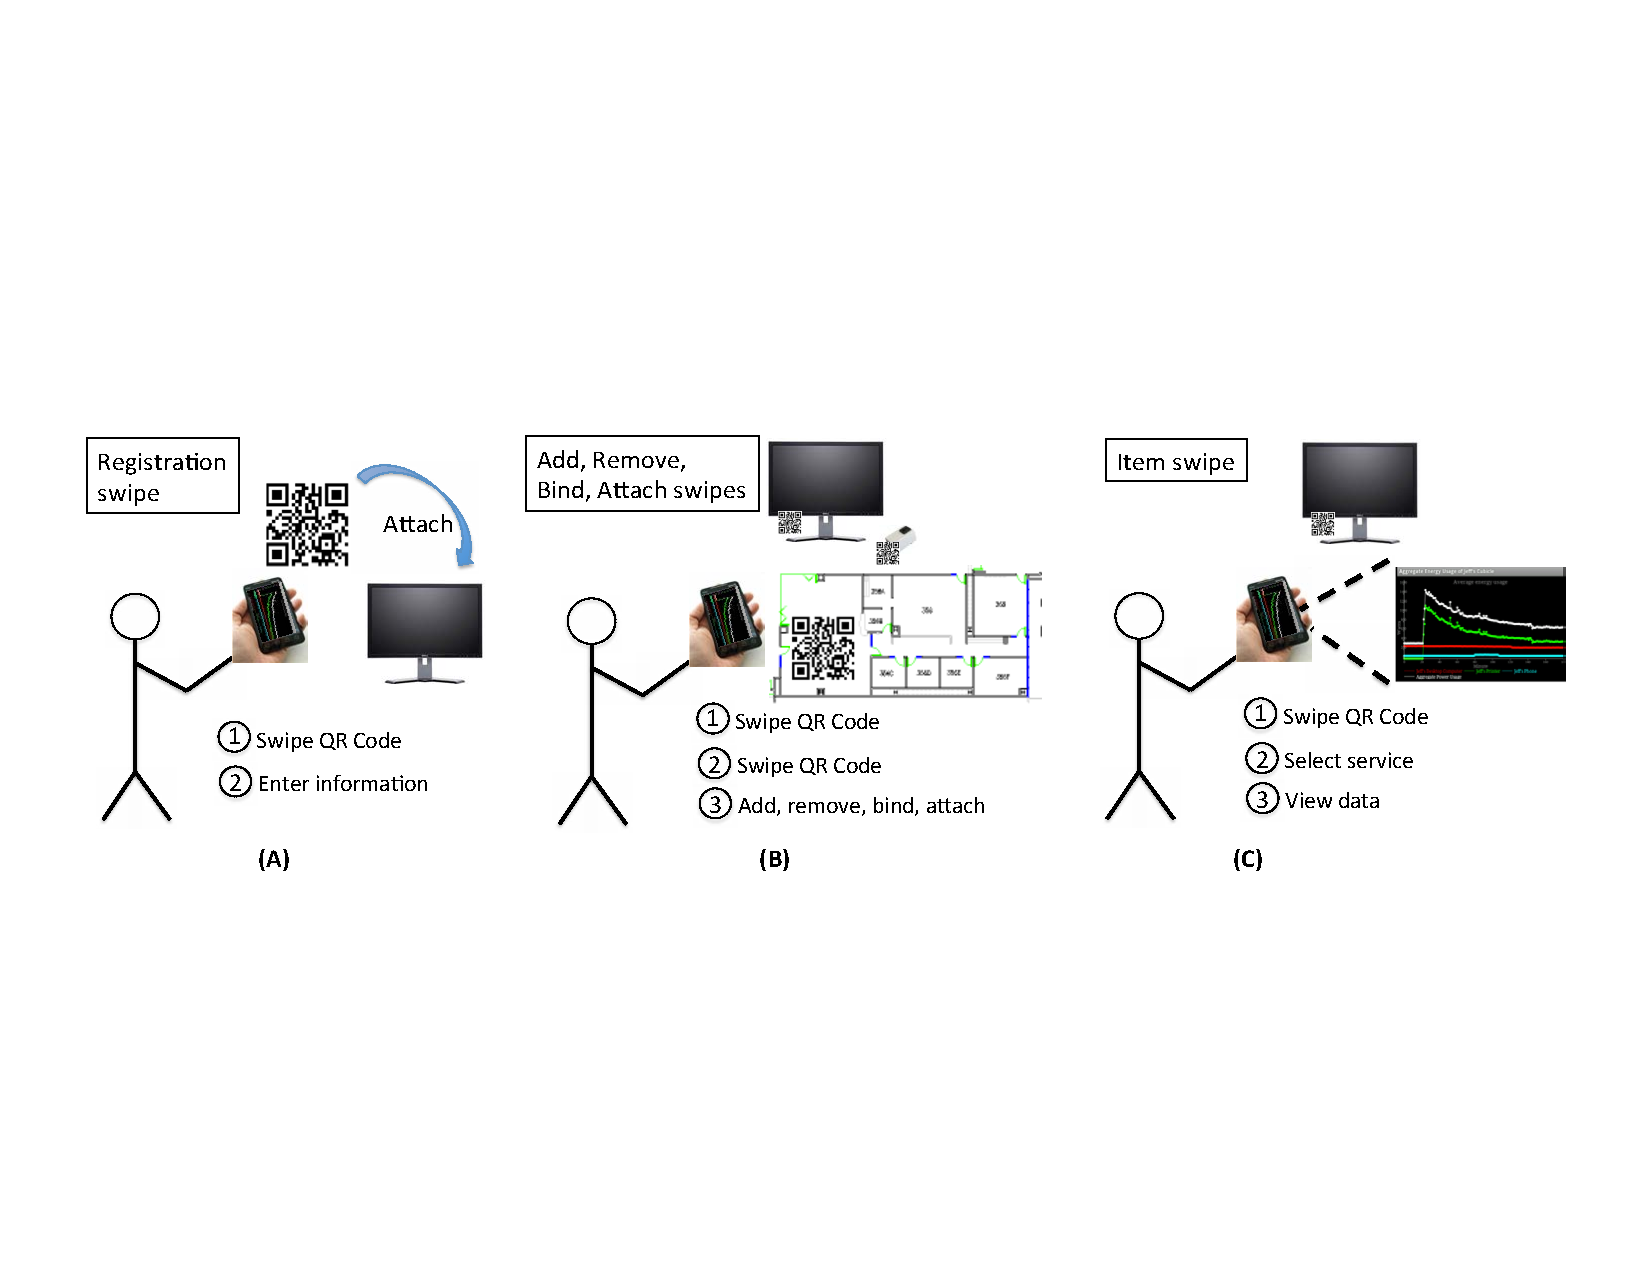
\includegraphics[width=\textwidth]{figs/swipes}
\caption{Gestures. Lorem Ipsum is simply dummy text of the printing and typesetting industry. Lorem Ipsum has 
been the industry's standard dummy text ever since the 1500s, when an unknown printer took a galley of 
type and scrambled it to make a type specimen book.  }
\label{fig:gestures}
\end{center}
\end{figure*}

\subsubsection{StreamFS}
\label{sec:streamfs}
%Discuss namespace management, binding, and recording data.
We used StreamFS~\cite{streamfs} as our data management layer.  StreamFS offers various
facilities to manage streaming sensor data and the associated metadata in a way that was useful for our the needs
of our application.  It organizes the metadata hierarchically and provides analytical
facilities that are baked into it, making it easier to create energy-analytics applications.  In particular,
StreamFS deals well with data aggregation where the number of constituents used to calculate the aggregate
changes over time.  In StreamFS, this is called \emph{dynamic aggregation} and it is described in more detail
in Section~\ref{sec:dynagg}.

Because we are fundmentally dealing with organizing data about the real-world, StreamFS is particularly useful over
a relational database abstraction.  StreamFS essentially constructs an entity-relationship graph~\cite{Chen76theentity-relationship}
and exposes this graph through a object pathnames and symbolic links.  It has been argued that semantic information
is lost in a relational data model~\cite{semanticmodel,semanticrelational}.  Our applications are built on
entity-relationship semantics, making StreamFS an ideal choice.

Each object in physical space is represented by a node in StreamFS.  Through StreamFS' RESTful/HTTP interface, we can
fetch the any node through a path rooted at the location where StreamFS is hosted.  For example, if we wish
to access the power meter in room 400 of building bldgXYZ, we may access it by issuing an HTTP {\tt GET} request to
{\tt http://server.streamfs.com/bldgXYZ/rm400/pow}.  The request returns a {\tt JSON} object with attribute-value
pairs that give a description of the temperature sensor.  It also returned that last received value from that sensor.
StreamFS provides a query interface to fetch the timeseries data collected from the sensor as well.

In addition, StreamFS support symbolic linking and this allows us to refer to nodes by multiple names.  That same 
power meter can also be referred to through {\tt /jortiz/meters/pow}; the meters that belong to user \emph{jortiz}.
More generally, StreamFS offers features that simplify namespace and data management.  Semantically, the hierarchical
node structure can be interpretted by the application.  We describe the structure and interpretation in
each application is section~\ref{sec:apps}.


\section{Gestures and QR code design}
This section briefly describes the basic primitives and design decisions that are used across all our applications.
The first is the set of gestures people perform with the smartphones to provide and obtain information about
the physical world.  The other describes our QR code design choices and why they are critical for engagement
and scalability.

\subsection{Gestures}
Mobile phones are very well engineered for incorporating natural gestures to acquire and view information.
We tried to take advantage of this by using simple gestures to obtain information about objects, context, and
movement.
Figure~\ref{fig:gestures} show the basic gestures to perform various actions.  The basic gestures fall into three
categories: registration, linking, and acquisition.  Registration is shown in the Figure~\ref{fig:gestures}(A).
It consist of a single tag swipe and entering information through the screen.  Linking gestures, 
shown is Figure~\ref{fig:gestures}(B), consist of
two swipes and the press of button to confirm the un/linking.  Finally, the acquisition swipe, shown
in Figure~\ref{fig:gestures}(C),  is a single swipe, select the data aggregate you wish to view, and viewing the data.

Each of these are natural for the user for capturing the physical world.  Swipes \emph{of}
the physical world are taken to tell us about something \emph{in} the physical world.  This makes the connection
clear to the user about the kind of information they are informing the system about.  In section~\ref{sec:apps}
we will show how gestures also tell us a just enough information to infer information about context and movement.
These gestures form the set of interaction primitives for all our
applications.  

The application logic associated with the gesture
defines the form of the relationship or action that is associated with the
gesture, such as {\tt is-in}, {\tt is-measured-by}, or {\tt
  get-control-of}.  This is in stark contrast to the use of gesture
recognition to infer actions that the person wants to perform on a
smart space.  The person takes a natural action, much like flipping on
a light switch, in order to perform an action or obtain information.
The scope of such actions is unconstrained because they are
interpreted by applications using the phone as a lens.

% \begin{itemize}
% \item Hierarchical organization
% 	\begin{itemize}
% 	\item building
% 		\begin{itemize}
% 		\item spaces
% 		\item inventory
% 		\end{itemize}
% 	\item symbolic links between spaces and inventory
% 	\item categorical
% 	\item users
% 	\end{itemize}
% \item Setting virtual view -- construction of the world
% 	\begin{itemize}
% 	\item Add/Remove through scan and input
% 	\item Un/Attaching
% 	\item Un/Binding
% 	\end{itemize}
% \item Setting context -- where in the world am i
% 	\begin{itemize}
% 	\item Check-in swipe
% 	\item Swiping items
% 	\end{itemize}
% \end{itemize}

\subsection{QR code design}
\label{sec:qrcodedesign}

An interesting observation we made in our deployments is that complex QR codes are difficult to capture and resolve
quickly, especially under poor lighting conditions.
The more data you encode on the QR code, the more 
intricate the pattern that is generated, therefore we tried to minimize the size of the {\tt URL} encoded on the QR code.  
Figure~\ref{fig:qrcexcomp} shows the difference between encoding a 
long %~\footnote{{\tt http://is4server.com/mobile/nokia/mobile.php?qrc=4eb46a8709e57}}
{\tt URL} to a short {\tt URL} shows an % http://tinyurl.com/6235eyw}.  Figure~\ref{fig:qrcexsecond} shows an 
example QR code that we used to tag items in one of our deployments.  Notice the difference between Figures~\ref{fig:qrcexfirst} 
and \ref{fig:qrcexsecond}.  The first QR code encodes 62 characters versus 26 characters for the second one.

% \begin{figure}[htb!]
% \begin{center}
% 
\includegraphics[scale=0.125]{figs/qrcexlong}
% \caption{This is an example QR code from our application. This label resolves to {\tt http://tinyurl.com/6235eyw}.
% We used tinyUrl to reduce the QR code image complexity and scan time.}
% \label{fig:qrcex}
% \end{center}
% \end{figure}

\begin{figure}[htb!]
\begin{center}
\subfigure[Long QR Code.]{%
            \label{fig:qrcexfirst}
            
\includegraphics[scale=0.148]{figs/qrcexlong}
        }
\subfigure[Minimized QR Code.]{%
            \label{fig:qrcexsecond}
            
\includegraphics[scale=0.35]{figs/qrcex}
        }
\end{center}
\caption{
	The QR code on the left resolves to the same {\tt URL} at the right one, after resolution and
	redirection is complete. 
	The short label resolves to {\tt http://tinyurl.com/6235eyw}.  The second encodes about half
	the characters as the first.
	We used tinyUrl to reduce the QR code image complexity and scan time.
     }%
\label{fig:qrcexcomp}
\end{figure}

\begin{table}
\label{tab:qrscans}
\begin{center}
  \begin{tabular}{| r | c  c | }
    \hline
    			 & {\bf Average (sec) } & {\bf Variance (sec)} \\ \hline
    Short,light & 1.66 & 0.33 \\ \hline
    Short, dark & 2.08 & 0.35 \\ \hline
    Long, light & 2.26 & 0.71 \\ \hline
    Long, dark & 2.82 & 0.50 \\
    \hline
  \end{tabular}
\caption{Shows the time to scan a long QR code versus a short QR code in light and dark conditions (loosely defined).
Notice that short QR codes scan faster and with less variance that long ones.}
\end{center}

\end{table}

Table~\ref{tab:qrscans} shows the results of some simple scanning experiment between the two tags
shown above.  We scanned each QR code under light and dark lighting conditions, off the screen of my laptop.
Each experiment was run 10 times and the table shows the statistical
overview of the results. 
Clearly, scanning the simple QR code under well-lit conditions
performed the best.  The complex QR code under the same condition takes about 28-36\% longer to scan.
On a generic QR code scanner, as used here, there is a portion of the
scan time that is independent of the code complexity.  As these are
more heavily used, this is expected to be reduced substantially and
the difference is acquisition complexity will be even more pronounced.
Perhaps even more important is the variance.  Notice that the variance with the simple QR code is much smaller and
more stable under either condition.  In our experience, {\bf large variance in scan time is a major
problem for complex QR codes}.  Thus we decided to re-design our codes and push more information in the lookup
processes, as network access was more reliable than the focus of the camera on various mobile devices.
Tags are placed on all types of devices in all kinds of locations with varying degrees of lighting.
Simple QR codes are vital for widespread use.

The design choice forced us to examine others that were related.  Not being able to encode much information on 
our QR codes means we are more reliant on the network to provide the bulk of the information, to be very reliable,
and to be widespread enough that disconnection is not problematic.  Moreover, there are a number of clients
that can be used to access and display the information and the tag has to be meaningful for both.
In order to meet these criteria we (1) shrunk {\tt URL}'s using tinyURL~\cite{tinyurl} as a level of 
indirection and 
(2) designed two classes of applications: \emph{shallow} applications, and \emph{deep-inspection} applications.  Shallow
applications interact with the web-application directly while deep-inspection application use
the {\tt URL} of the web application to extract a unique identifier and provide deeper inspection
and update capabilities of the entity-relationship graph.

An example {\tt URL} we used in our deployment is {\tt http://tinyurl.com/6235eyw}.
When this is resolved, we get an empty response in the body, but we use the header to identify the QR code identifier 
that we associate with the item.  The response header looks as follows:
\begin{figure}[htb!]
\begin{center}
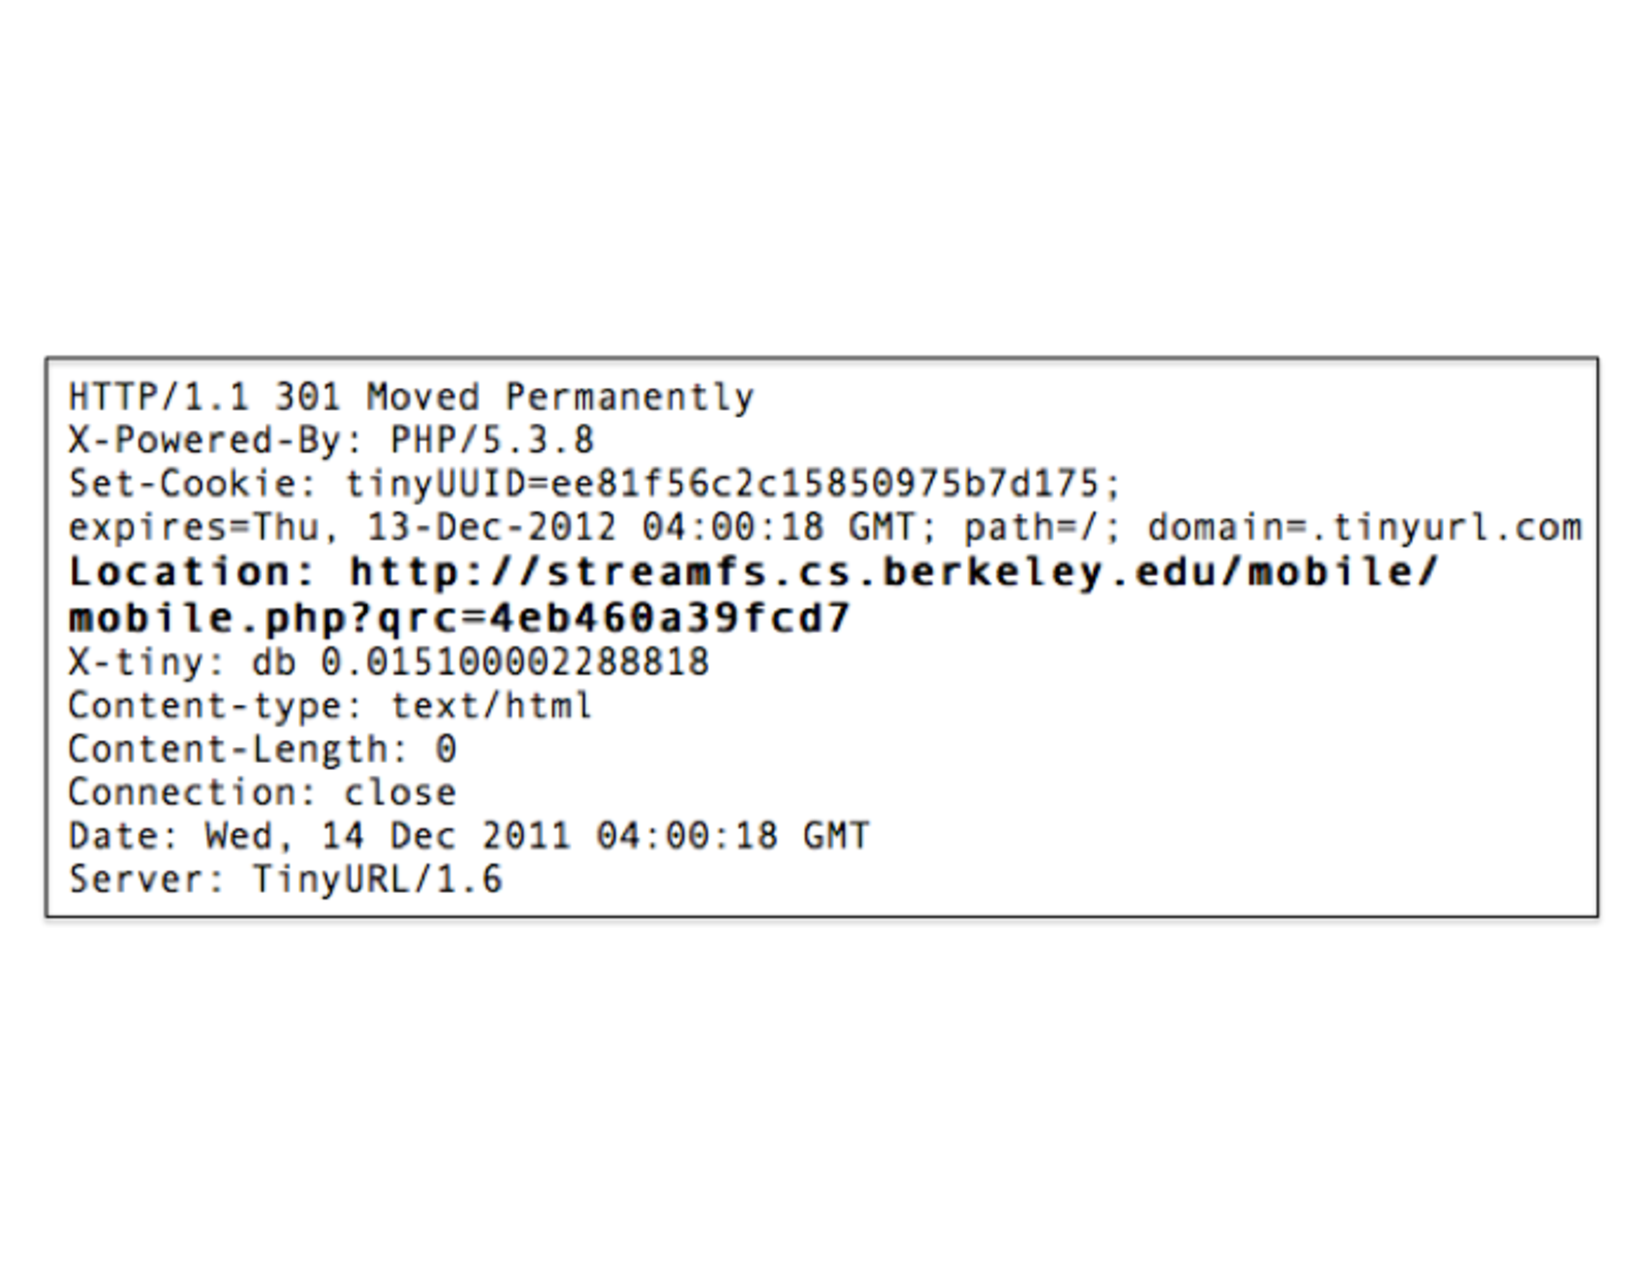
\includegraphics[scale=0.30]{figs/tinyurlhdr}
\caption{The header of the response from the {\tt tinyUrl} when resolving a QR code.  The `Location' attribute
is used to extract the unique identifier for the object this QR code tags.  It is also used to re-direct
users without the phone application to a meaningful web address for the object.}
\label{fig:tinyurlhdr}
\end{center}
\end{figure}

% It provides a web address for users to re-direct to and find information and various read-only services for the object.  However, because
% the {\tt URL} also contains a unqiue identifer \emph{qrc}, it can be used to provide for sophisticated services and capabilities.
% An example is the ability to change the virtual structure of inter-relationship between this object and other objects.  This
% is demonstrated in our energy auditing application discussed in detail in section~\ref{sec:eaudit}.
% Once items are tagged, they can be added and removed by swiping the tag and pressing the button for what you want to do with
% the item.  You also check into locations either explicit with a location-tag swipe or implicitly with an item swipe.

Notice the `Location' attribute in the header.  This is the location of the re-direct.  \emph{Shallow} applications
use the {\tt URL} directly.  The \emph{qrc} {\tt URL} is unqiue identifier for the item that this tag is attached to.
A shallow application can obtain mostly read-only service through our web applications.  For example, we'll see how
to get either item-specific data or item-aggregated data with respect to the user making the request (i.e. the total
energy consumed by \emph{my} devices).  \emph{Deep-inspection} applications are native to the phone, so we can do much
more with the tag.  Our energy auditing application allows you to related the item to other items by maintaining state of swipe
history.  This is more difficult with the web-applicaiton.  We can also use the tag and item information to couple it with
sensor information coming from sensors on the phone itself.  For example, we could determine the direction an object
is pointing by using the phone's directional sensor and negating their direction (i.e. phone is facing east, tag on item must
be facing west).








\section{Applications}
\label{sec:apps}
% In this section we discuss three applications we wrote that use the infrastructure we set up inside a building on campus.
% The building is a 7-story, 141,000 square-foot building.  We tagged 351 items spread over 139 rooms throughout all floors.
% There are WiFi access point spread throughout the entire building, providing ubiquitous access to a network throughout.
% Cellular coverage is also available throughout most of the building as a secondary option for connecting to a network.

In this section we discuss three applications deployed on top of our infrastructure.
The first is an energy auditing application.  The goal of the application is to quickly collect,
organize, and understand plug-loads, also known as miscellaneous
electrical loads (MELs), in the building.
The application provides scalability of the inventory collection process where there previously was none.
Various governmental agencies have conducted field studies of this
sort in order to characterize these loads, but they are severely
limited by the effort involved in obtaining the
inventory\cite{***http://www.efficientproducts.org/reports/plugload/Revised_Office%20Plug%20Load%20Report_PIER_500-06-007_RevApril2011.pdf
                                stevel}. 
 And, the inventory quickly becomes stale as items are moved and
 changed, further frustrating longitudinal studies.  Our goal is not
 just to facilitate the field studies but to make the audit a natural
 offshoot of using the appliances such that it can be used as part of
 an organization energy management strategy without expertise in
 energy auditing.
A second-order result of the audit in the infrastructure it leaves deployed.  We used the deployment
to implement two more applications.  The energy item scanner application gives historical energy information
for any item that the user swipes.  Items include physical objects \emph{and} spaces. Since spaces do not directly 
consume energy, they embody notion of an aggregate.
Similarly, personal energy metering embodies the notion of an aggregate or a family of aggregates.  That is
our the third application we present.

For each we discuss the fundamental challenges with respect to mobility, consistency management, or aggregation and how
our use of gestures and interference were used to address these issues.  We also discuss how the underlying entity-relationship
graph is used to deal with a dynamic set of constituents when computing aggregates.

% We collected both power rating information as well
% as live metering information.  The second application, the energy-view item scanner, builds off the first, allowing users
% to swipe the QR code of an item and view the power-trace and power-rating recorded for that item.  It is also
% used to view aggregates across space; you can scan a floor and see the aggregate data for that floor over time.  
% The third is a personal energy accountant.  This application allows users to virtually tag items that belong to them 
% and view their personal energy consumption, aggregated across all the devices they own.

\subsection{Energy Audit}
\label{sec:eaudit}
Nationally, MELs consume about third of the energy in building in the United States~\cite{eia:2010}.  However,
given the nature of these electrical loads, collecting enough information quickly from hundreds of disparate
loads spread throughout the building simply does not scale.  In~\cite{lbnlmels}, they describe the major challenge
in collecting device inventory for studying MELs and state the the process simply does not scale to large buildings.

The energy audit application addresses this issue.  We leverage the occupants, particularly the ones with mobile phones
to scale the inventory collection processes.  Once they download our application and print a QR code from our site, they
attach it to an item and register it using the phone.  This scales to any building size, as long as the number of occupants
scales with the number of devices and the size of the building.

Execution of the audit builds the entity-relationship graph.  Each time a new item or space is registered a node is added
to the graph.  The first objects we need to learn about are spaces and how they are inter-related.  StreamFS
was pre-populated with a directory to record that information.  A user can add a new room if either the room has no tag
or the current tag is not registered (which they can determine by swiping it).  Once a room is added, objects within that
room can be added.  Figure~\ref{fig:msfsv2} shows a screen shot of the auditing application.  
We also applied a classification hierarchy on the objects using a MELs taxonomy~\cite{taxonomy}
incorporated into StreamFS as a directory.

Note, however, that in order to add an object, we need to know where you are.  That is the main piece of contextual information
that must be deduced or reported.  Prior work has used indoor WiFi~\cite{radar}, learning-based approach~\cite{wigem}, 
and alternative infrastructure~\cite{cricket}.  However, we took a simpler approach:

\begin{enumerate}
\item The person swipes into a space, setting it as their conext for adding new objects or
\item They swipe an, whose location we already know, and we use that to infer their current location.
\end{enumerate}

This approach is much simpler than prior work, but just as effective.  
% It also involves the user in the check-in process rather
% than the infrasture learning about the user.
% It also empowers the person to get involved
% in processes, forcing them to think about the energy problem through explicit participation in the use of the application.


%Restering an object or space adds a node to the entity-relationship graph that represents the physical state of the world.  
%Because each of the physical object are spread throughout the building, 
%maintaining consistency is fundamentally hard and unscalable without occupant participation.  
%In addition, in constructing the relationship graph, the main piece of information is where the object is in the building.  

% To start we need to capture the objects and relationship between them.  Specifically, we set up the hierarchical organization of
% objects with the building at the root, followed by \emph{spaces} and \emph{inventory} within the building, and data streams at the leaves.
% The spaces subtree is the hierarchical organization of floors, rooms, and areas on those floors.  The inventory is a folder where
% each of the physical objects is placed.  We used symbolic links to associate items in the inventory with the location
% they are in.  In addition, we added a categorical subtree to ease aggregation with respect to the category of devices.
% For personalized accounting, users created their own folder that points to items that belong to them.
% Figure~\ref{fig:hierarchy} shows a partial view of the hierarchy that supports our applications.

% After the hierarchy is constructed, we place QR codes on objects in the world and register them.  The registration process
% for locations includes the following steps:

% \begin{enumerate}
% \item Place QR code somewhere in the space.
% \item Scan QR code.
% \item Choose which space it represents.
% \end{enumerate}

% \vspace{0.04in}

% The basic set of spaces that initially inputted by hand are the building and the floors.  We placed QR code on the entrance of the building
% and the main door to enter the floor.  Once each of these spaces is registered, the user can set their context by swipe the QR code tag.
% When rooms are added, the user first scans the tag for the floor they are on, then they place a tag on the room and they enter information
% about the room.  For items, the process is the same.  We scan the room we are in, place the tag on the object and enter information about
% object.

% The initial location scan sets the context.  For example, when you first enter a building, you scan the QR code associated with that building.
% The {\tt URL} fetched from the QR code is first resolved.  

\subsection{Inter-relationship capture}
\label{sec:binding}
%Talking about how you bind an item and meter.
There is a special relationship between meters and items.  Items are attached to meters, but more importantly, the data
collected from the sensor \emph{represents} the underlying dynamics of some physical measurement related to the item.  A power 
meter attached to a television gives us the power profile of that television over some time period.  Furthermore, if the meter 
is removed
from the television and attached to another item, that change needs to be recorded, so that we do not attribute the power
trace from the second item to the television.  There are also items are that attached to each other that can affect how we 
aggregate feeds.  For example, in our deployment, we sometimes connect meters to power-strips, which have multiple items
attached to them.  The meter serves as a proxy-aggregate for the attached the power strip that's attached the meter.

%FILL IN WITH REAL GRAPH
\begin{figure}[htb!]
\begin{center}
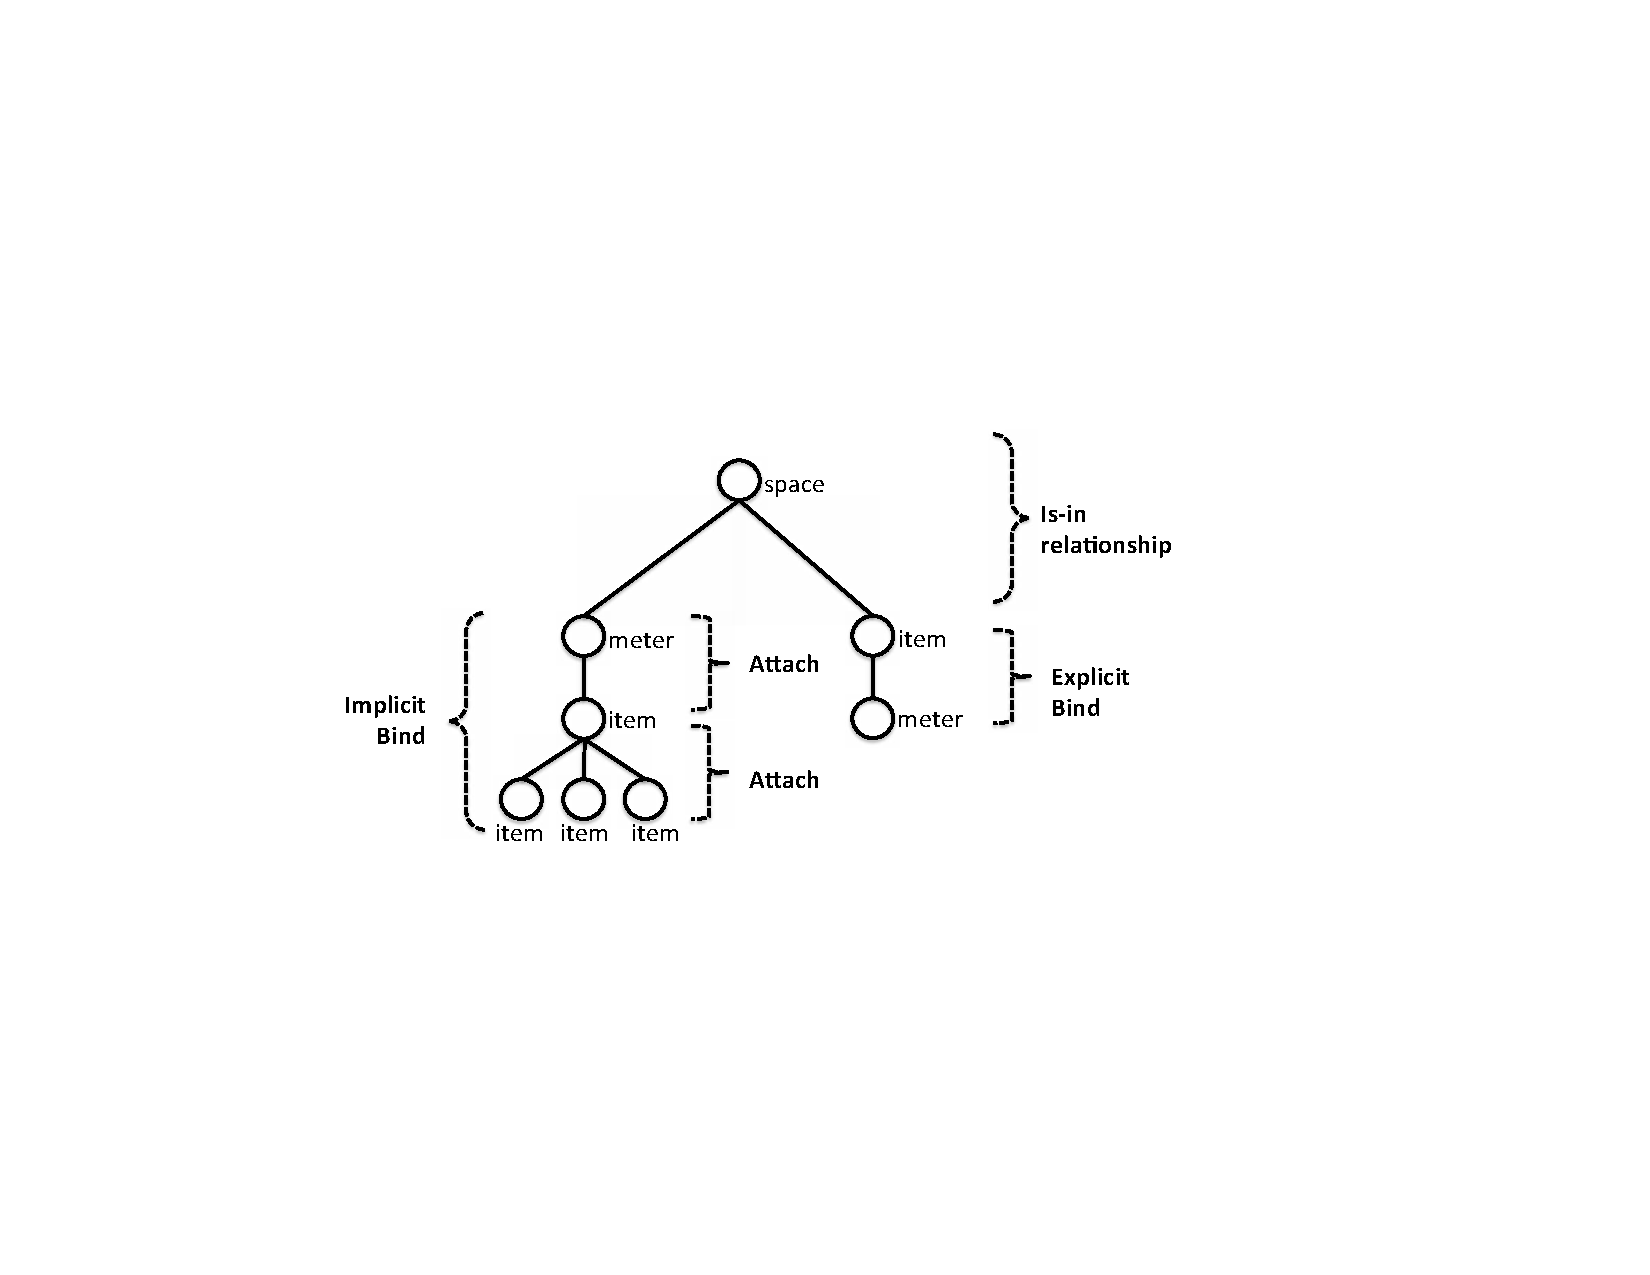
\includegraphics[scale=0.55]{figs/bindattachstructs}
\caption{This diagram shows the relationship capture between the objects and locations in the building for the 
energy audit application.  Children of a space node have an ``is-in'' relationship with the space.  An item
with another item as a child have a ``attached'' relationship and meters attached to items are bound to each other.
Note, this is a \emph{subset} of the relationship diagrams generated across our three applications.}
\label{fig:attachandbind}
\end{center}
\end{figure}

Both types of relationship are interpretted by how nodes are symbolically linked.  If a meter is the child
of an item, it is bound to that item and can be used as a proxy for measurements pertaining to that item.
If an item is a child of a meter, it is attached to the meter, but the measure is not taking measurements
pertaining to the item, instead if it taking measurement of the children of the item.  Figure~\ref{fig:attachandbind}
highlights the two kinds of relationships interpretted by our applications.  The one of the left shows
a bind relationship while the one of the right shows and attach relationship.
To bind or attach the gesture is the same.  You first swipe the item the swipe the meter and press a button to either
un/attach or un/bind.

% \subsection{Energy Auditing}
% The energy auditing application was written to capture all of the plug-load devices in a building.  Included it their
% capture is information about the plated power-draw of the device, if available, its make, model, and category.
% The capture consists of walking around the building with a set of QR codes, registering each of the rooms and items
% within them.  For each room you enter the name of the room.  The floor is indicated explicitly through a swipe of the buidling
% floor tag.  Once inside the room each electrical device is tagged and registered.  To register the item the QR code needs
% to be added, followed by a small form that is filled out by the auditor.  The form includes information for the name
% of the device and the power rating or current draw.  

Figure~\ref{fig:msfsv2} shows two screenshot of the auditing interface.  The first page is a list of options and the second is
the registration page.  Once the page is filled out, the user scans the QR code once again and the item is added to the inventory.
In addition, the QR code tag identifier is added to the `qrc' directory and symbolically linked to the newly added item
in the inventory directory.  Finally, a symbolic link is create in the directory for the room that also points to the item
just added to the inventory.

\begin{figure}[htb!]
\begin{center}
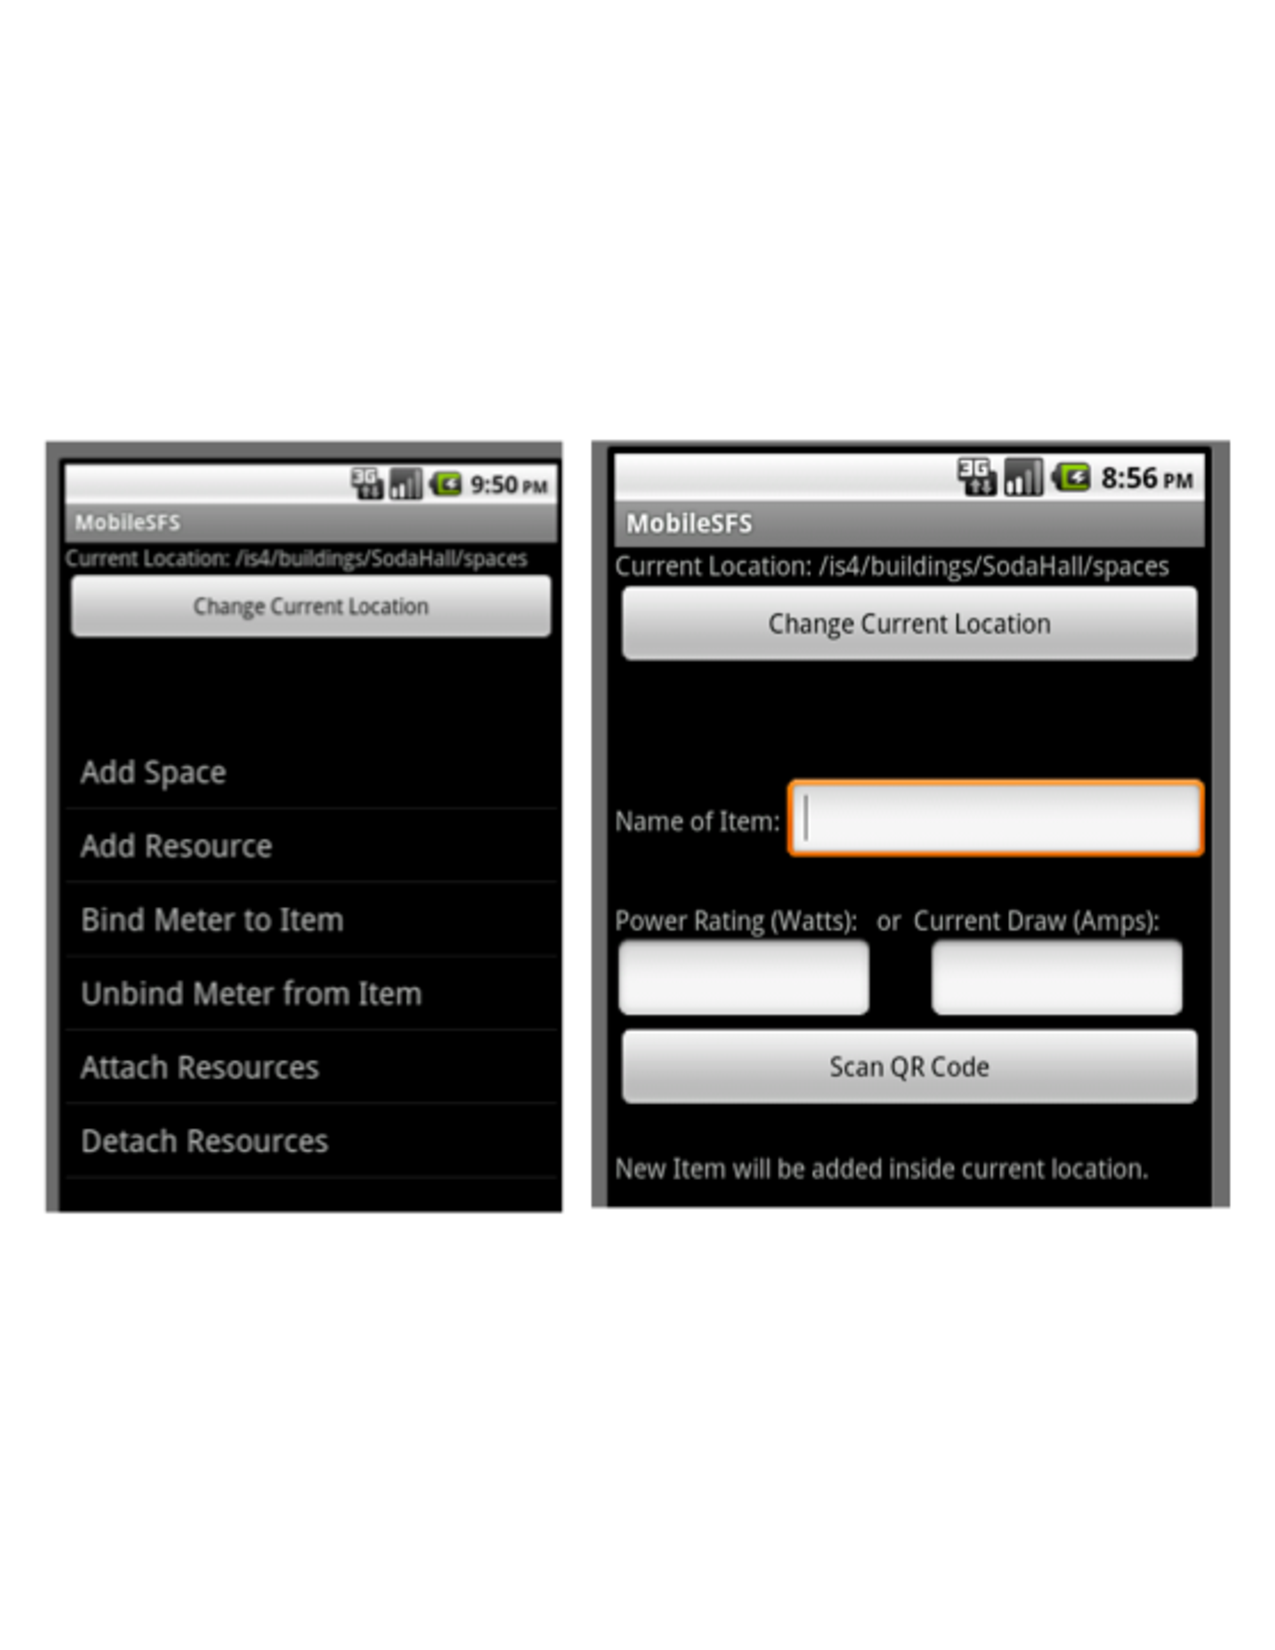
\includegraphics[scale=0.39]{figs/msfsv2screens}
\caption{}
\label{fig:msfsv2}
\end{center}
\end{figure}

Auto-classification was done using the same of the item as well.  In addition to the spaces, qrc, and inventory directories
there is also a taxonomony directory.  Items with a given prefix were classified as being items in a particular
directory of the taxonomy.  A symbolic link was also created from the corresponding node in the taxonomy, that most closely
matches the item, to the item node.

In our current deployment we use the link gesture to link an appliance
to the wireless power meter that monitors its consumption.  In the
future, such capability might well be built into the appliance
itself.  However, other contextual information about the appliance and
its relationship to the space and the people that use the space is
likely to remain.

\subsubsection{Results}
This application was focused on capturing the physical, energy-consuming objects, describing them in various way
and coupling that information with live streaming power data.  Figure~\ref{fig:devicecount} shows the breakdown of the
types of devices that were recorded by the energy auditing application.  Since this data was collected from a office
building, most of the device were actually LCD screens.

\begin{figure}[htb!]
\begin{center}
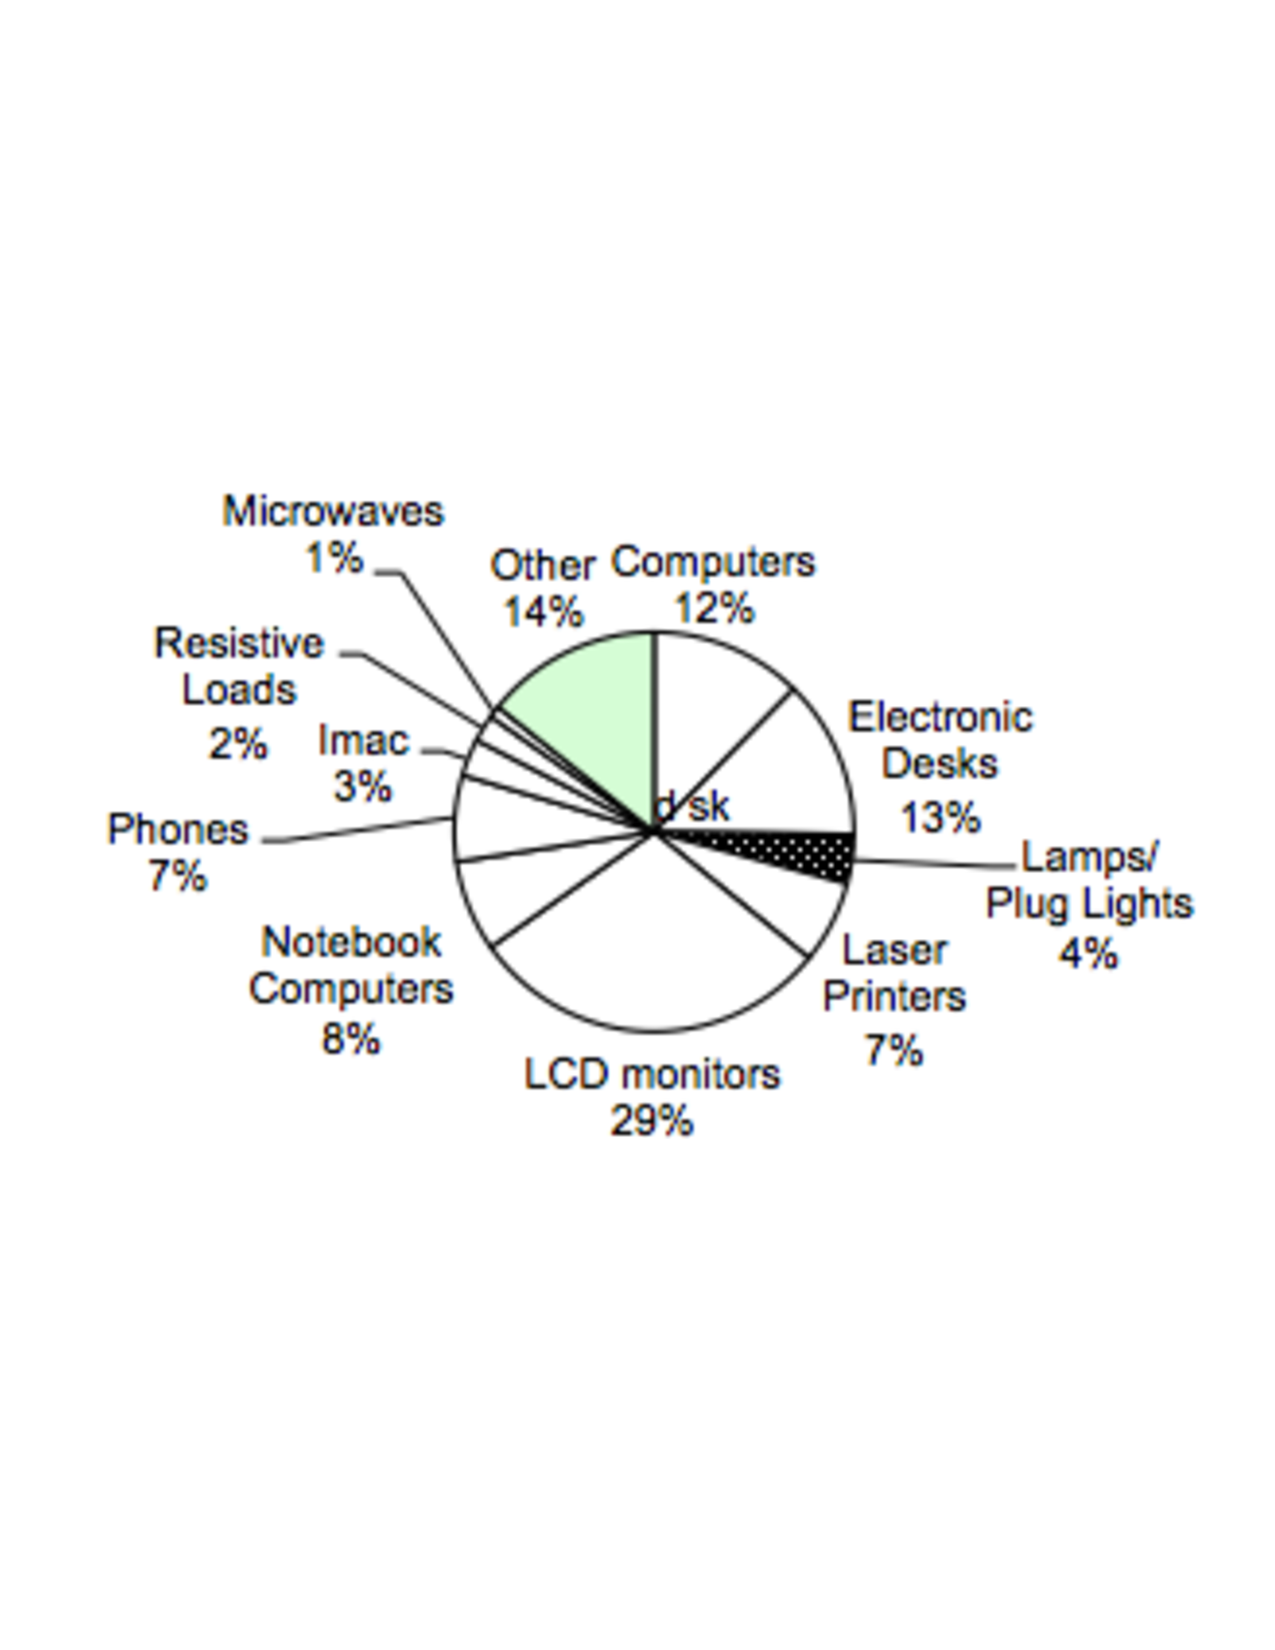
\includegraphics[scale=0.42]{figs/devicecount}
\caption{The percentage breakdown of the devices that were captured.}
\label{fig:devicecount}
\end{center}
\end{figure}

Although most of the items are static, a good number of them are moved by their owners pretty often.  For example, 8\%
of the device were classified as notebooks.  When the owner leaves the room or building, they usually take their notebook
with them.  This kind of information should be recorded using the auditing application.  By simply swiping QR code for the notebook
and clicking the `leave' button, the item is kept in the inventory for the building, but the symbolic link from the 
room to the item is deleted.

\begin{figure}[htb!]
\begin{center}
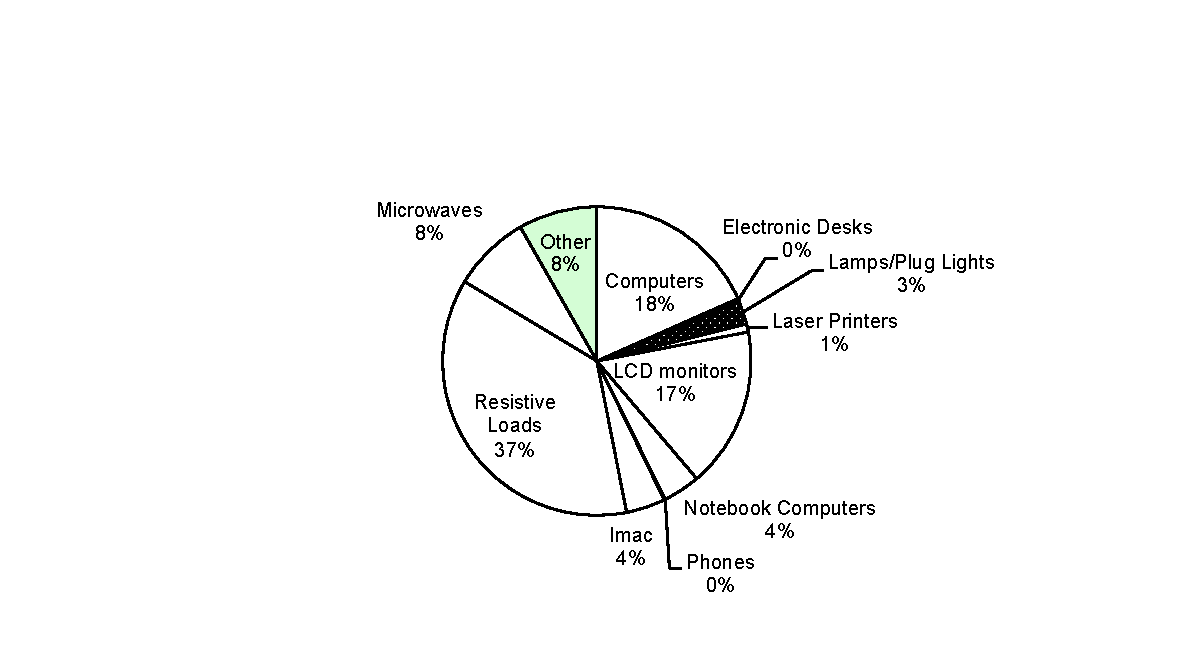
\includegraphics[scale=0.7]{figs/PIE_CHART_SANS_WATTS}
\caption{Device power draw in Watts.}
\label{fig:piechart}
\end{center}
\end{figure}

Figure~\ref{fig:piechart} shows the power-draw distribution.  Interestingly, although the category of devices that 
fall under `resistive loads', which includes things like space heaters
and toaster ovens, make up only 2\% of the items recorded, they
account for a much larger fraction of the total power-draw.
% Axed the bogus stuff about multiplying something by nameplate.  It
% all depends on usage cycle anyways.  At best hope this gets in and
% this cruddy stuff gets fixed.  Currently it is totally bogus


\begin{figure}[htb!]
\begin{center}
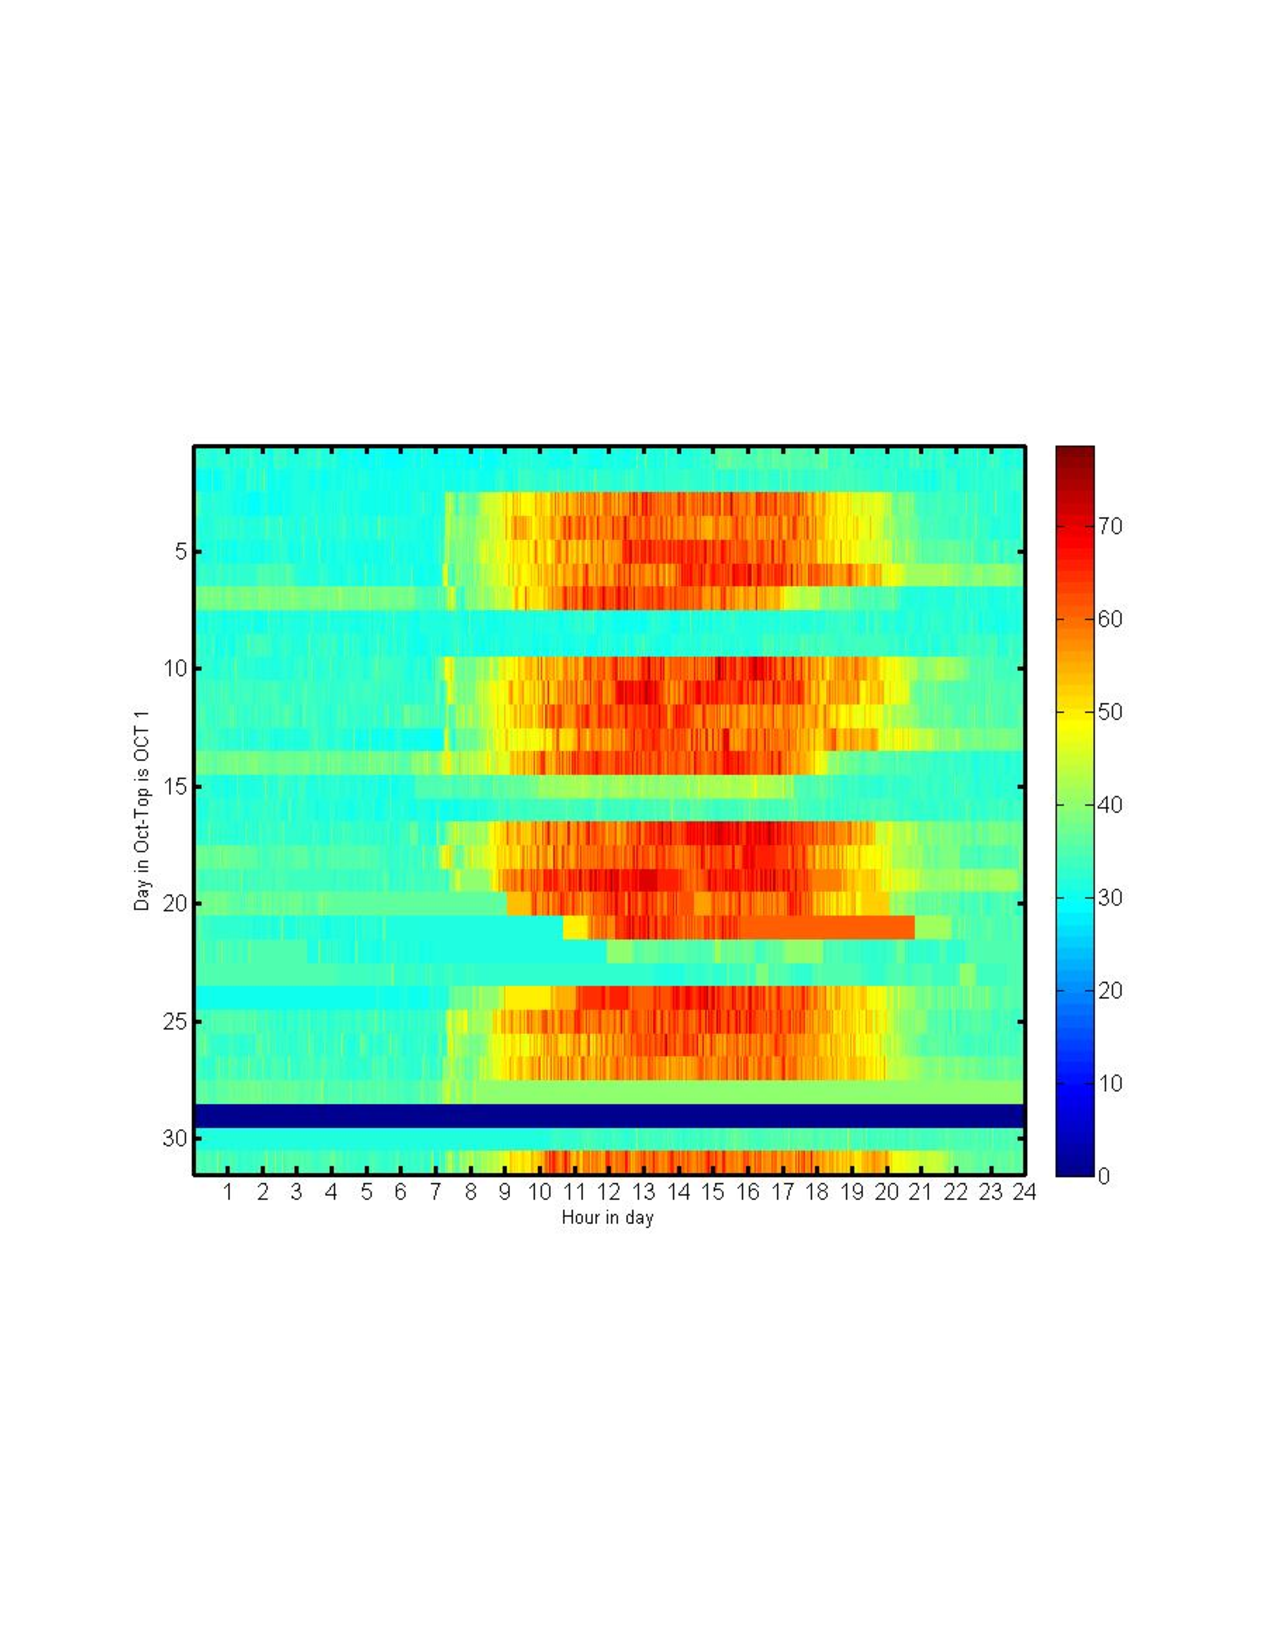
\includegraphics[scale=0.49]{figs/Aggregate_SDH_OCT_PLUG_LOADS}
\caption{Power heatmap generated from the data obtained from meters attached to plug-load devices throughout the building.  
Red zones are locations where the highest amount of power is being consumed.}
\label{fig:plugloadheatmap}
\end{center}
\end{figure}

Figure~\ref{fig:plugloadheatmap} was generated using actual live, plugload data throughout the day during the entire month
of October.  The x-axis shows the hour of the day, while the y-axis indicates the day in october.  This data was aggregated
over hourly period by summing all the plug-load data collected over that hour.  Notice the busiest times between 10am and 
about 6pm.  There's also a clear view of the weekends.

% \begin{figure*}[htb!]
% \begin{center}
% 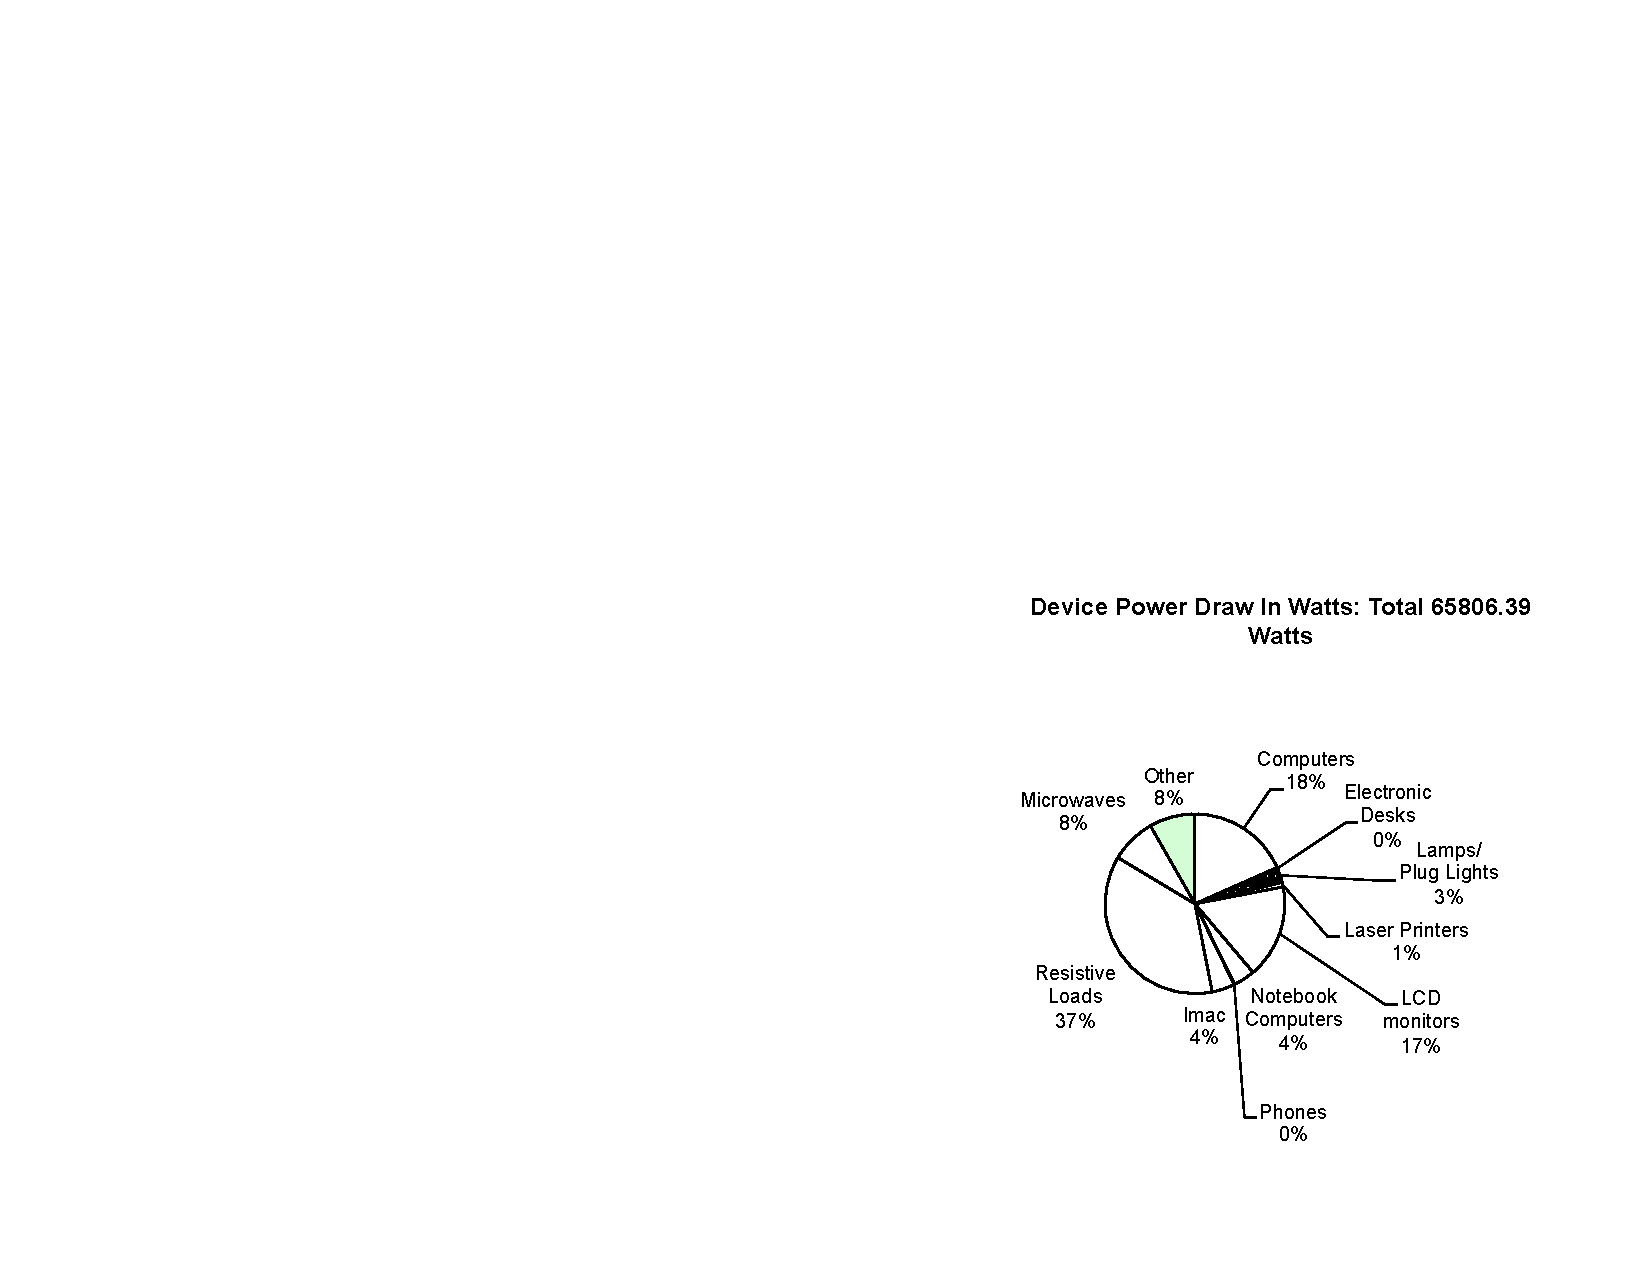
\includegraphics[scale=0.8]{figs/device_info02}
% \caption{}
% \label{channelcomp}
% \end{center}
% \end{figure*}

\begin{figure}[htb!]
\begin{center}
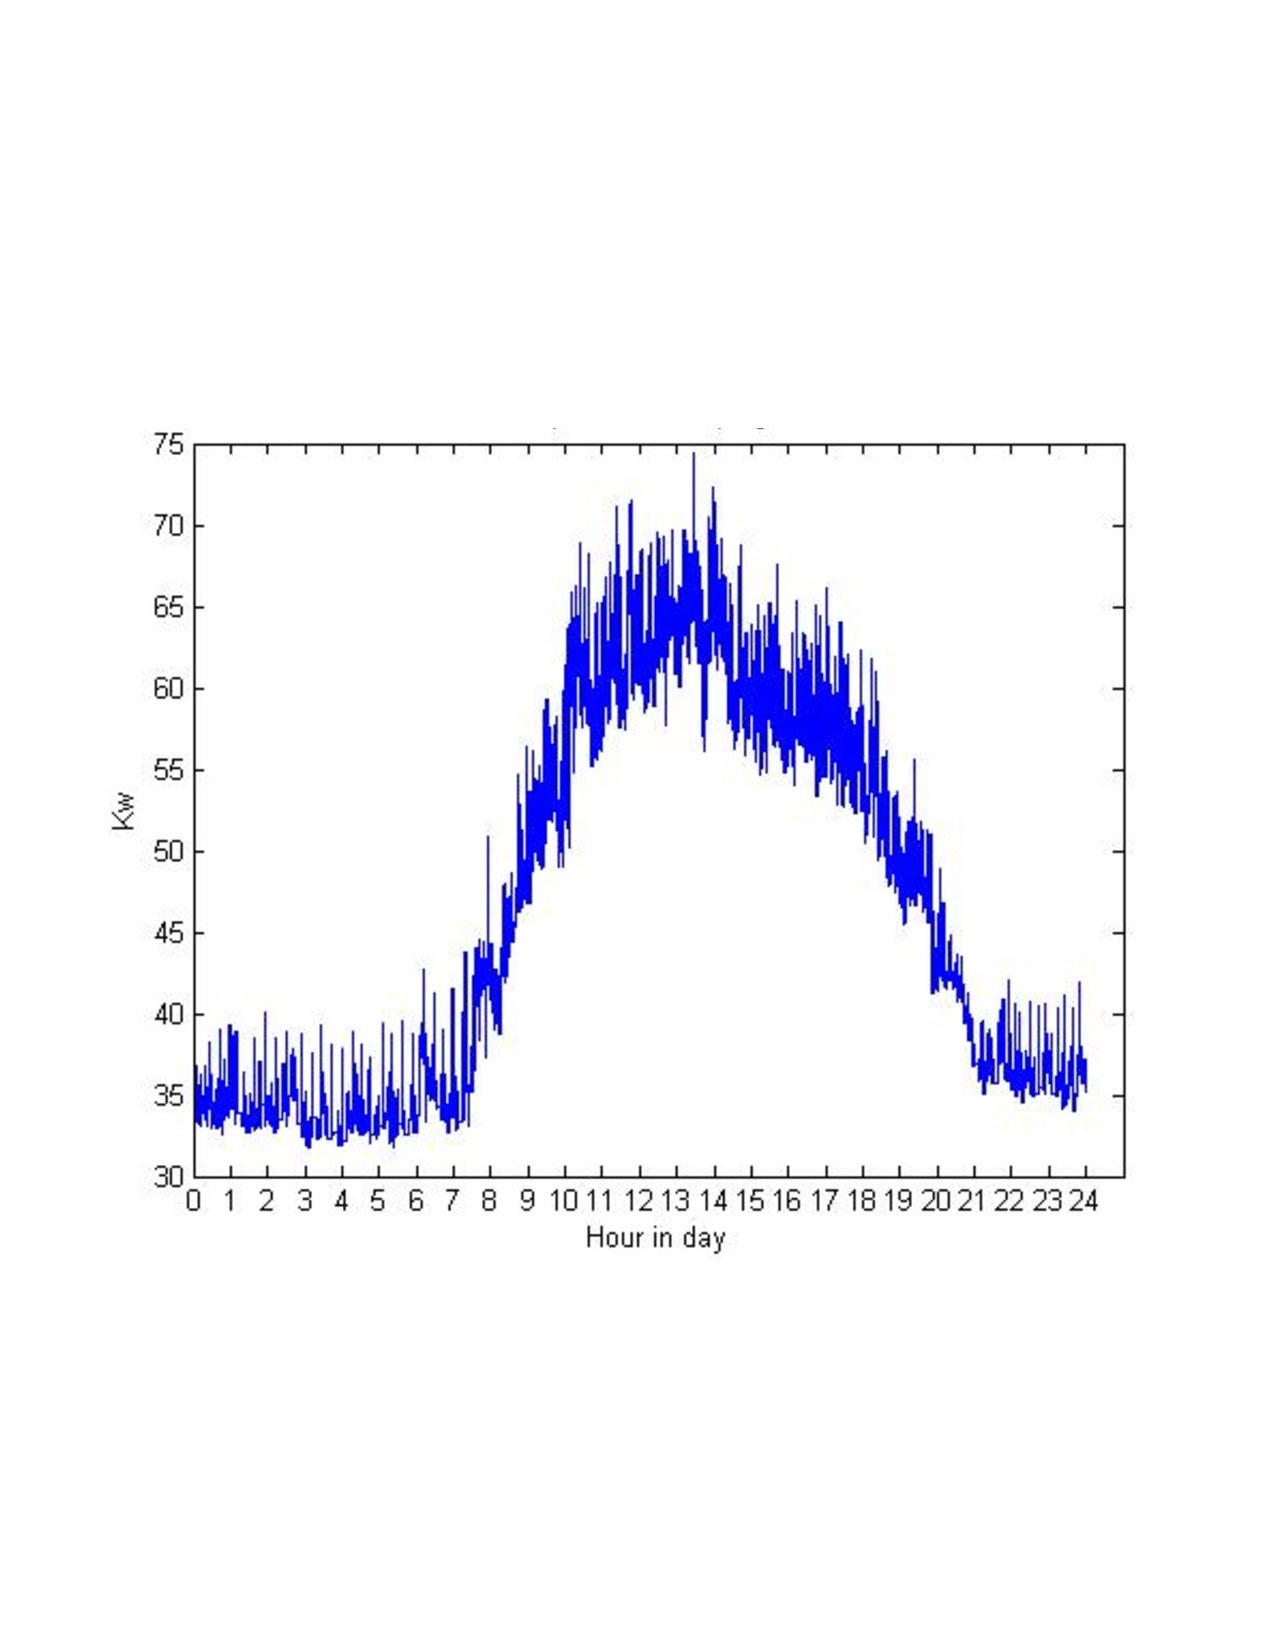
\includegraphics[scale=0.4]{figs/WholeOct12}
\caption{Whole building power draw on October 12th.}
\label{fig:wholebuilding}
\end{center}
\end{figure}

Figure~\ref{fig:wholebuilding} shows the whole building power-draw feed.  This meter was obtained through the building
management system and added to the audit.  Notice how the peak and low times correspond to the patterns observed
in the monthly plug-load heat map.

% \begin{figure}[htb!]
% \begin{center}
% 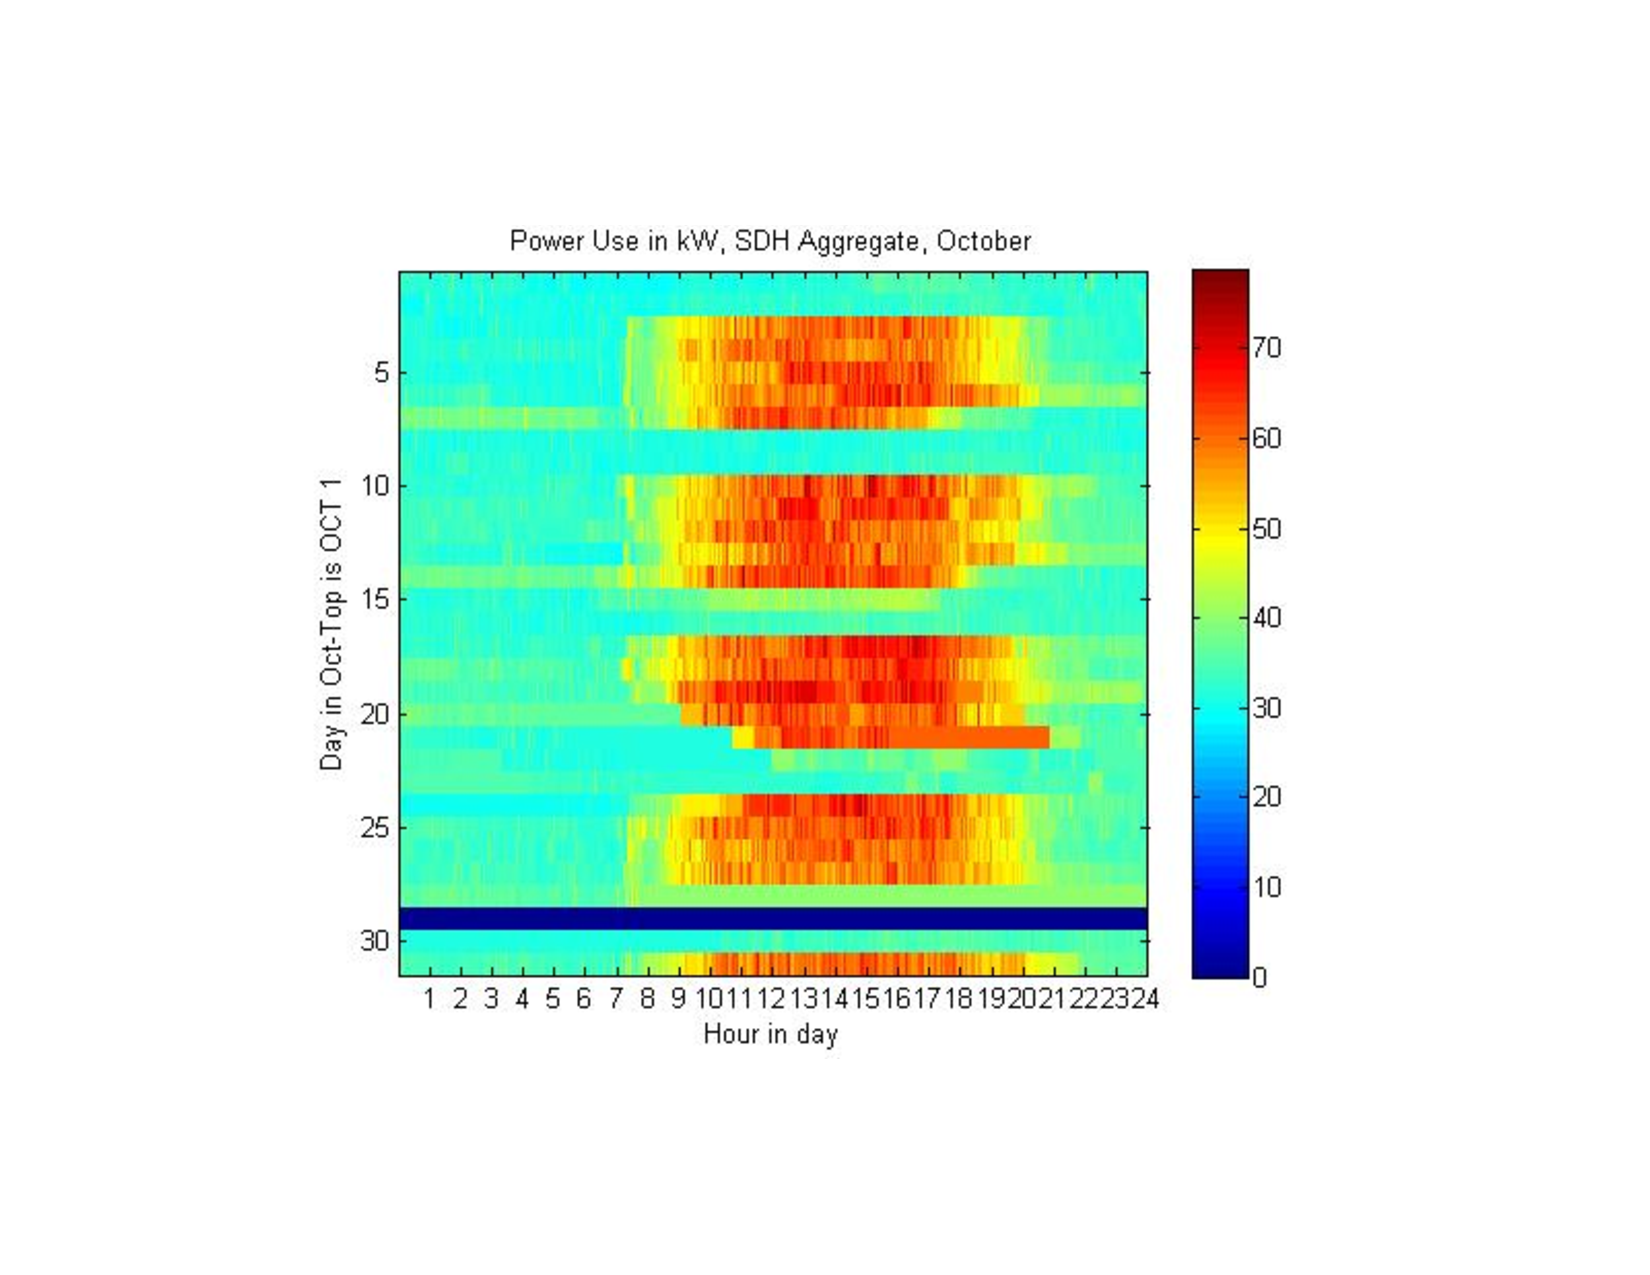
\includegraphics[scale=0.4]{figs/heatgrid}
% \caption{}
% \label{channelcomp}
% \end{center}
% \end{figure}

\begin{figure}[htb!]
\begin{center}
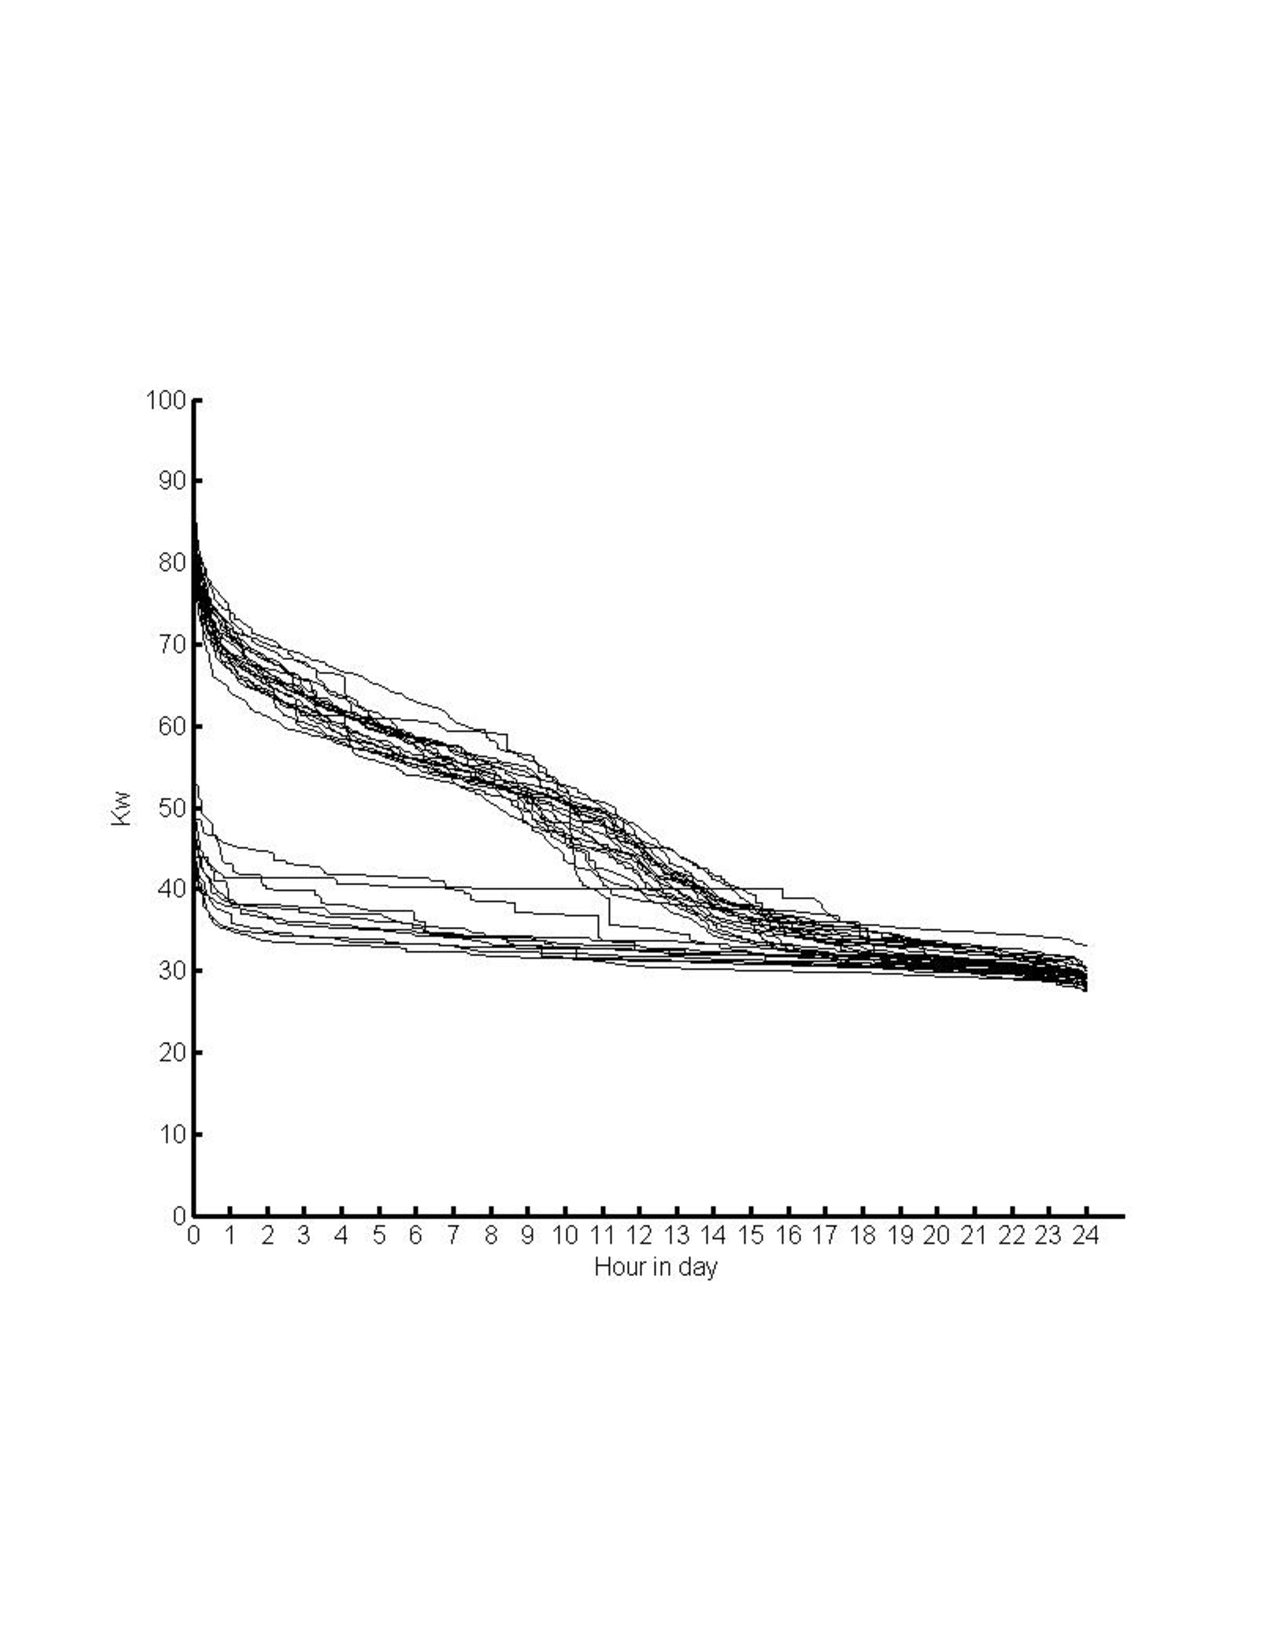
\includegraphics[scale=0.4]{figs/LoadDurationCurvesWholeBuildingBLACK}
\caption{Load duration curves.}
\label{fig:ldc}
\end{center}
\end{figure}

Figure~\ref{fig:ldc} shows the load duration curve for each day in the month of October.  The load duration
curve shows the number of hours in a 24-hour day that the load was at or above the level indicated on the 
y-axis.

\subsubsection{Issues}

Although many of the calculations are static and in large aggregates there were some fundamental challenges that
we encountered.  The first challenge is maintaining \emph{consistency} between the physical world and the virtual
representation of it.  About 16\% of the plug-load items we registered can be moved between locations by they owner
with relative frequency.  7\% (laptops) move quite often.  Maintaing of accurate view of what items are where
is a non-trivial with the right mechanisms in place.  Our approach in this case is to depend on the ubiquity of
smartphones and participants.  If a person moves an item from one location to another, they can swipe the item out
of the current location and swipe the item back in at the new location.  In addition, we take advantage of
natural usage patterns.  People tend to forget to swipe items out of their current location, so we leverage the
second swipe (swipe-in) to imply the first operation (swipe-out).  If the item was connected to a meter, we unbind the item
from the old meter before swiping the item out.  

We are currently working on adjusting the timestamp based on this action as well.
From the trace of the meter we can see when the item was unplugged (or turned off).  The sudden drop in power
reading could be used to mark the point of disconnection.  However, this only gets us part of the solution.  If the person
forgets multiple actions, it become more difficult to determine what has occurred.  For example, if a lamp is plugged
into a meter in room 1 and they unplug it from the meter, plug another device into it, and move the lamp to
another location, the unplug time is not clear.  If the new device draws power, we cannot tell the difference between
the trace generated from the new device versus the old device.  This is a non-intrusive load-trace classification
problem and beyond the scope of the current project.

% \begin{itemize}
% %\item Context tracking:  Localization through a swipe or implicit location change through natural action
% \item tracking mobile users
% \item tracking mobile objects
% 	\begin{itemize}
% 	\item devices
% 	\item meters
% 	\end{itemize}
% \end{itemize}
\subsection{Item Scanner Application}
The next two application were built on top of the deployed infrastructure from the energy audit.
The item scanner application shows a power trace of an item.  If the item is a space, it shows
the aggregate consumption of the space over a 24-hour period.  Figure~\ref{fig:itemscanscreen}
shows a screenshot of a trace for a room in on of the spaces we monitored.

%FILL IN WITH REAL GRAPH
\begin{figure}[htb!]
\begin{center}
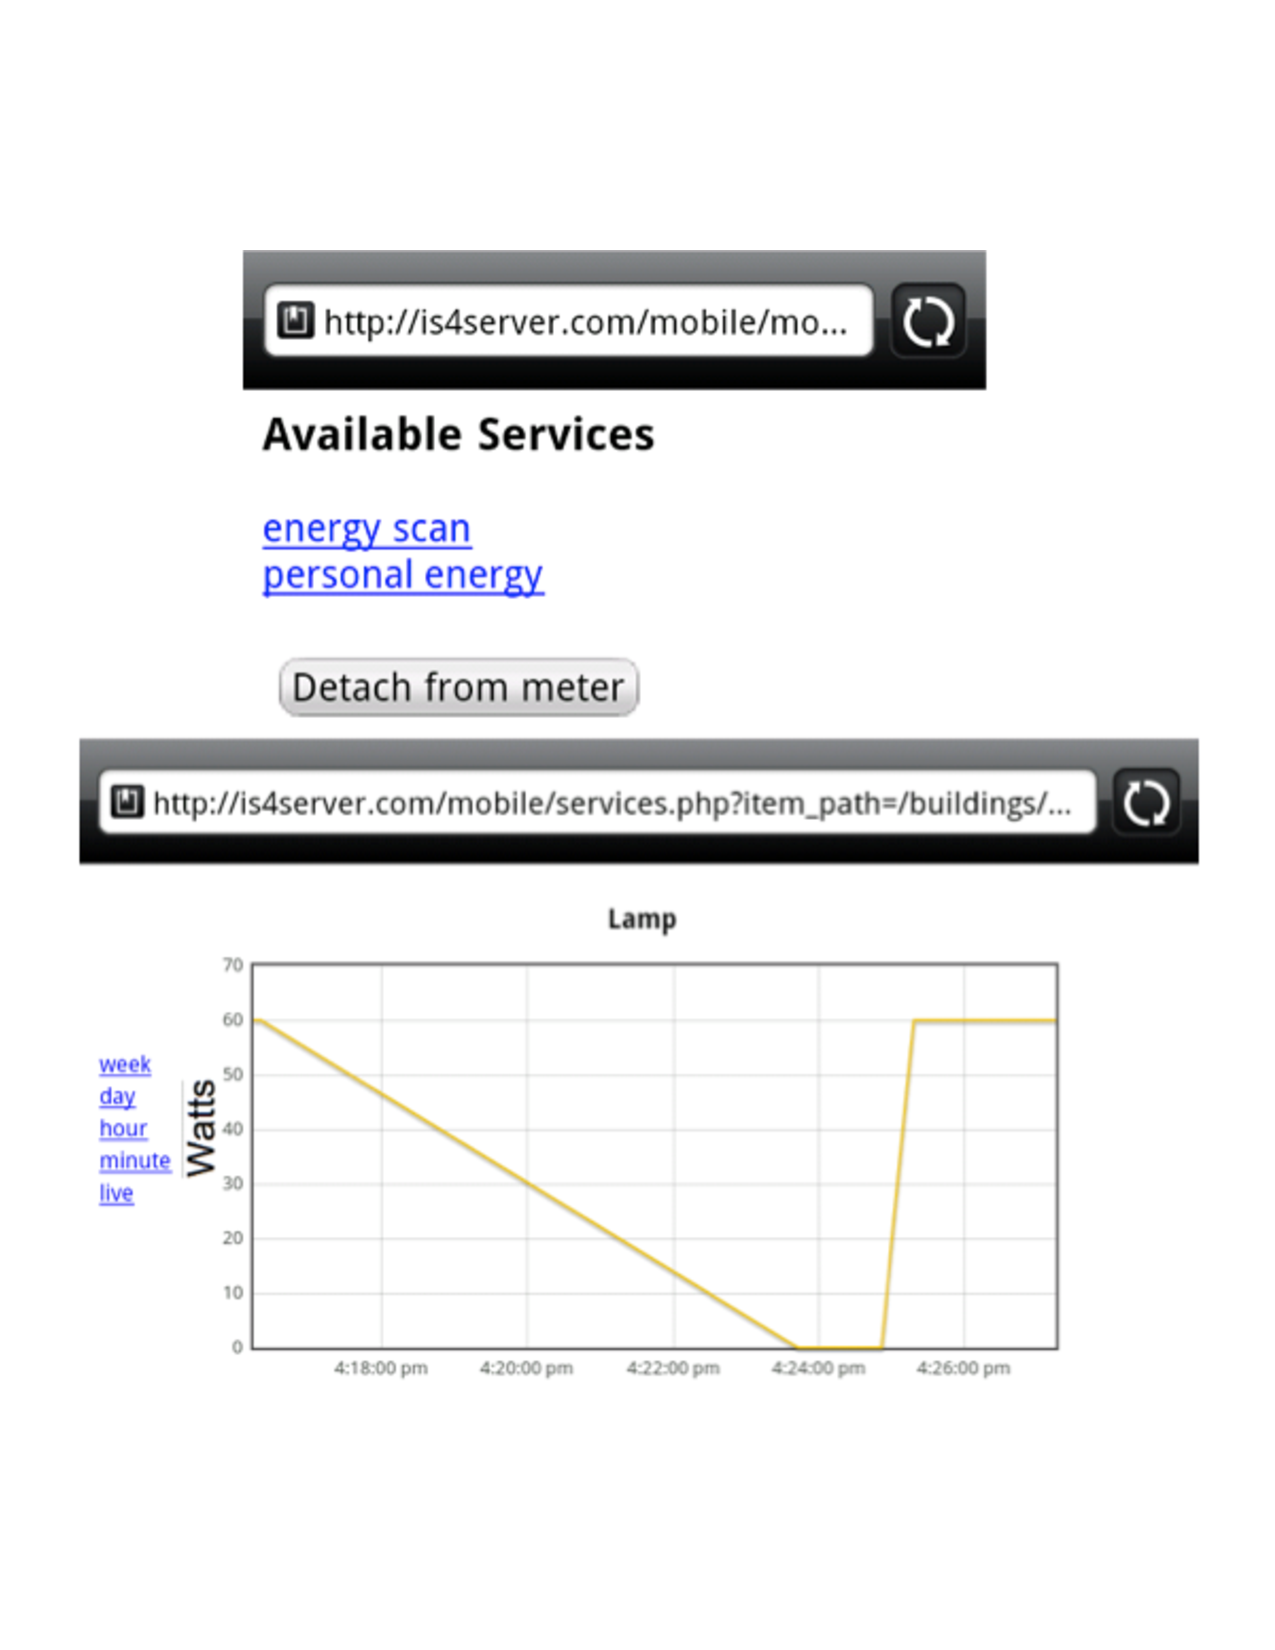
\includegraphics[scale=0.39]{figs/menuenergyscan}
\caption{Item scanner screenshot. Lorem Ipsum is simply dummy text of the printing and typesetting industry. Lorem Ipsum has 
been the industry's standard dummy text ever since the 1500s, when an unknown printer took a galley of 
type and scrambled it to make a type specimen book.  }
\label{fig:itemscanscreen}
\end{center}
\end{figure}

The main thrust of this application revolves around aggregating feeds with respect to the spatial hierarchy that was
constructed for the energy audit.  A person can scan any item from the building and floor down to the room
and individual device.

\subsubsection{Issues}
In addition to the consistency challenges from the energy audit, apportionment is non-trivial.  Even with an accurate
view of where items have been moved, tracking the consituents and calculating aggregate is challenging in real-time.
Since meter clocks are not syncrhonized, the data must be cleaned before an aggregate can even be computed.
We address this problem with dynamic aggregation and discuss the details in section~\ref{sec:dynagg}.

\subsection{Personalized Energy Tracking}
A user identifies themselves with a username and password.  This create a folder in StreamFS with their username.  As they
walk around the building, they can tag items that belong to them by swipe them and clicking `my item' in the mobile
application.  The application records the item and its location when this is done.  A location folder is created
in the user's directory along with a symbolic link to the item that they tagged.  This allows us to aggregate both the totals
by location and totals by user.  Figure~\ref{fig:personalscanscreen} shows the interface for tagging a device 
and the aggregate for the owner of the items.

%FILL IN WITH REAL GRAPH
% \begin{figure}[htb!]
% \begin{center}
% 
\includegraphics[scale=0.39]{figs/blankbox}
% \caption{Personal energy screenshot. Lorem Ipsum is simply dummy text of the printing and typesetting industry. Lorem Ipsum has 
% been the industry's standard dummy text ever since the 1500s, when an unknown printer took a galley of 
% type and scrambled it to make a type specimen book.  }
% \label{fig:personalscanscreen}
% \end{center}
% \end{figure}

\subsection{Issues}
In this application, the main challenge was in localization of a particular user.  In order to form aggregates for the total c
onsumed by the user in a particular sapce, we want to present the user with an aggregate of the items they know in that space.  
To do this automatically one might require indoor localization using the WiFi infrastructure.  However, we leverage the tags infrastructure
and user input to identify who they are and where they are.  With a simple `login' and swipe, they get personlized,
location-specific, aggregate energy consumption data.

\begin{itemize}
\item Mobile objects: objects move and are placed in different locations
\item Changing meters: meters are moved or items are disconnected and re-connected to other meters
\item Aggregation that track constituents over time:  just a description, talk more about it in next section
\end{itemize}
\section{Dynamic Aggregation}
\label{sec:dynagg}
Dynamic aggregation combines the underlying entity-relationship graph with in-network aggregation.  It treats
each node in the graph as a potential point of aggregation on a particular data type.  For example,
if we need to compute aggregates of \emph{KW} data and we declare the node for a particular room as
the point of aggregation, we accept data from all children of that node that, whose units are in \emph{KW},
and add the streams together over pre-defined window size or pre-defined timeouts.

The scheme is hiearchical, so a node only accepts data from its children and only sends data to its parent.
StreamFS checks for cycles when before node insertion and prevents double-counting errors by only allowing 
aggregation-points that are roots of a tree that is a sub-graph of the entity-relationship graph.  In our deployment,
each view is a managed as an independent hierarchy.  So the hierarchy of \emph{spaces} is separate from
the \emph{inventory} hierarchy or the \emph{taxonomy} hierarchy.  This allows us to ask questions with a particular
view in mind, without conflict, and is a natural fit for our aggregation scheme.

\subsection{How it works}
Although there are different semantics applied to different node types at the application layer, StreamFS only knows
about two types of nodes: (1) default nodes and (2) stream nodes.  The main difference is that \emph{default} nodes
are not explicitly associated with data coming from a sensor and \emph{stream} nodes are.  Furthermore, default
nodes can have children, while stream nodes cannot.  In our application, meters are represented by default nodes
and each stream of data they produce is a stream node.

When an aggregation point is chosen and enabled, dynamic aggregation places a buffer at the node for the type
of data that should be aggregated.  If we want to aggregate \emph{KW} data, we specify the type and send an enable-aggregation
request to the node through an HTTP {\texttt POST} to the path for that node.  The flow of data starts at the leaves when
a stream node received data from a sensor through HTTP {\texttt POST}.  As data arrives it is immediately
forwarded upstream to the parent(s).  If a node that receives data from its children is an aggregation point it buffers
the data, otherwise it fowards it to its parent.

Ignoring the timeouts for now, lets imagine the parent is a point of aggregation and its buffer is full.  At this point
the parent separates data into bins for each source and cleans it for aggregation through interpolation.  The main
operation is to \emph{stretch} and \emph{fill} that data with linearly interpolated values.  The \emph{stretch}
operation orders all the timestamps in increasing order and for each bin (signal) interpolates the values using the
first (last) pair of data points.  If there is only a single data point, the stretch uses it as the missing value.
The \emph{fill} operation find the nearest timestamps that are less-than and greater-than the missing sampling time, 
uses their values to determine the equation of a line between them and interpolates the missing value using that equation.
Once this is done for each signal, the values are added together for each unqiue timestamp and the aggregated
signal is reported to the parent, where the operation occurs recursively to the root.
Figure~\ref{fig:aggtree} shows an illustration of its operation.  

%problem:  the buffer size has to increase exponentially up the tree, in order to not drop any values.
%solution: chuck the data into default-buffer sized pieces and parallelize the interpolation using the interpolated tasks technique


%FILL IN WITH REAL GRAPH
\begin{figure}[htb!]
\begin{center}
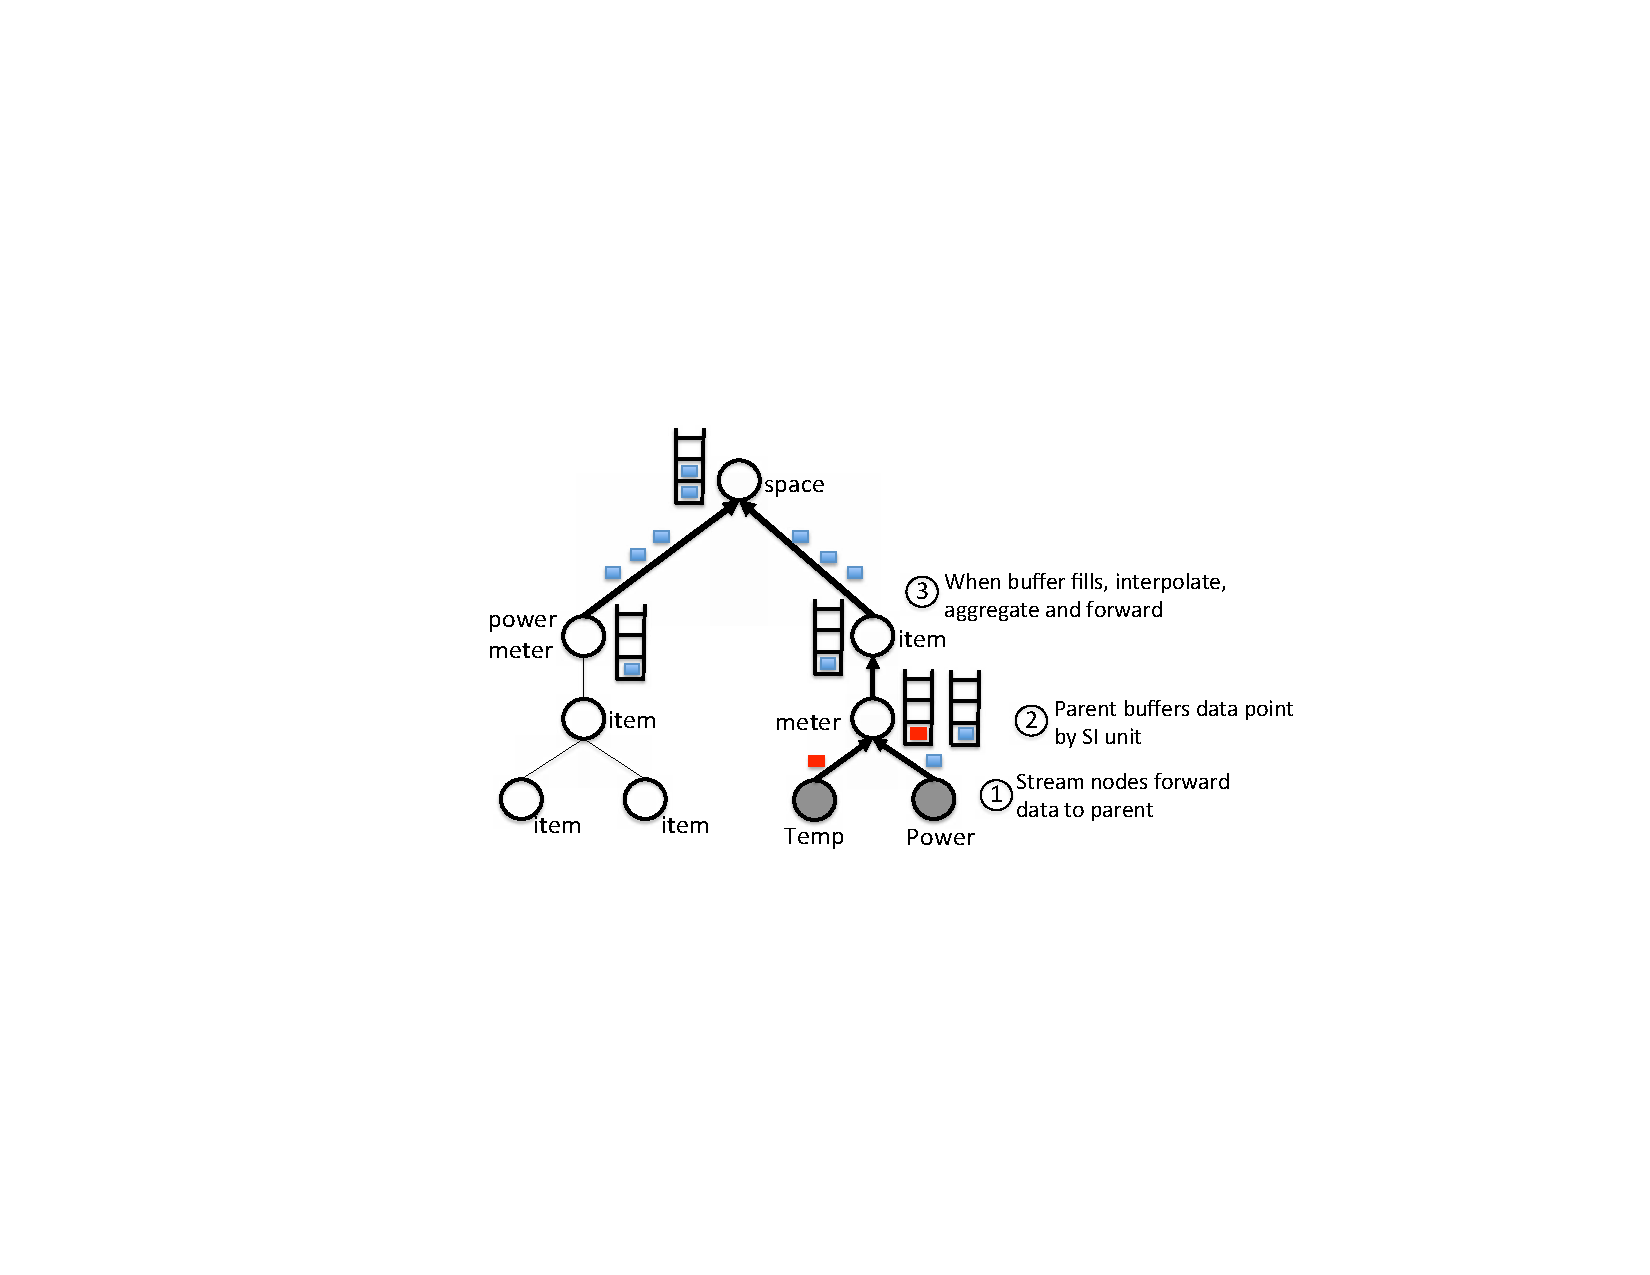
\includegraphics[scale=0.6]{figs/aggtree}
\caption{This shows an illustration of the aggregation tree used by \emph{dynamic aggregation}.  Data flows from 
the leaves to the root through user-specified aggregation points.  When the local buffer is full the streams
are separated by source, interpolated, and summed.  The aggregated signal is foward up the tree.}
\label{fig:aggtree}
\end{center}
\end{figure}

\subsubsection{Dealing with dynamics}
This approach deals with changes in the graph quite naturally.  All aggregation point deal only with local data, so
a node is only concerned about the children that give it data and the parent to send data to.  As objects in the environment
move from place to place and these changes are captured, the entity-relationship graph also changes to reflect the move.
This change in aggregation constituents is naturally accounted for in the aggregate.  If a child is removed,
it no longer forwards data to the old parent, therefore the aggregate will reflect that change.
Note, however, that changes in the entity-relationship graph are indistinguishable from energy-consuming items that have
been turned off.  For the purposes of aggregation, that is okay.

\subsubsection{Two scenarios}
We illustrate dynamic aggregation with a common usage scenario.  Imagine there are a number of people in a building,
each owning a number of plug-load applicances and a laptop.  Assume that when a person is in a room their laptop
is plugged in and when they leave the room they unplug their laptop and take it with them.  People come and go
throughout the day, changing the aggregate power consumption of the room and it happens.  In addition, some
of those people move to other rooms and plug their laptop in the new location.  As this happens, we will assume
all actions are being recorded in StreamFS.

%FILL IN WITH REAL GRAPH
\begin{figure}[htb!]
\begin{center}
\subfloat[Room 1 object and aggregate streams.]{%
            \label{fig:dynaggs1room1}
            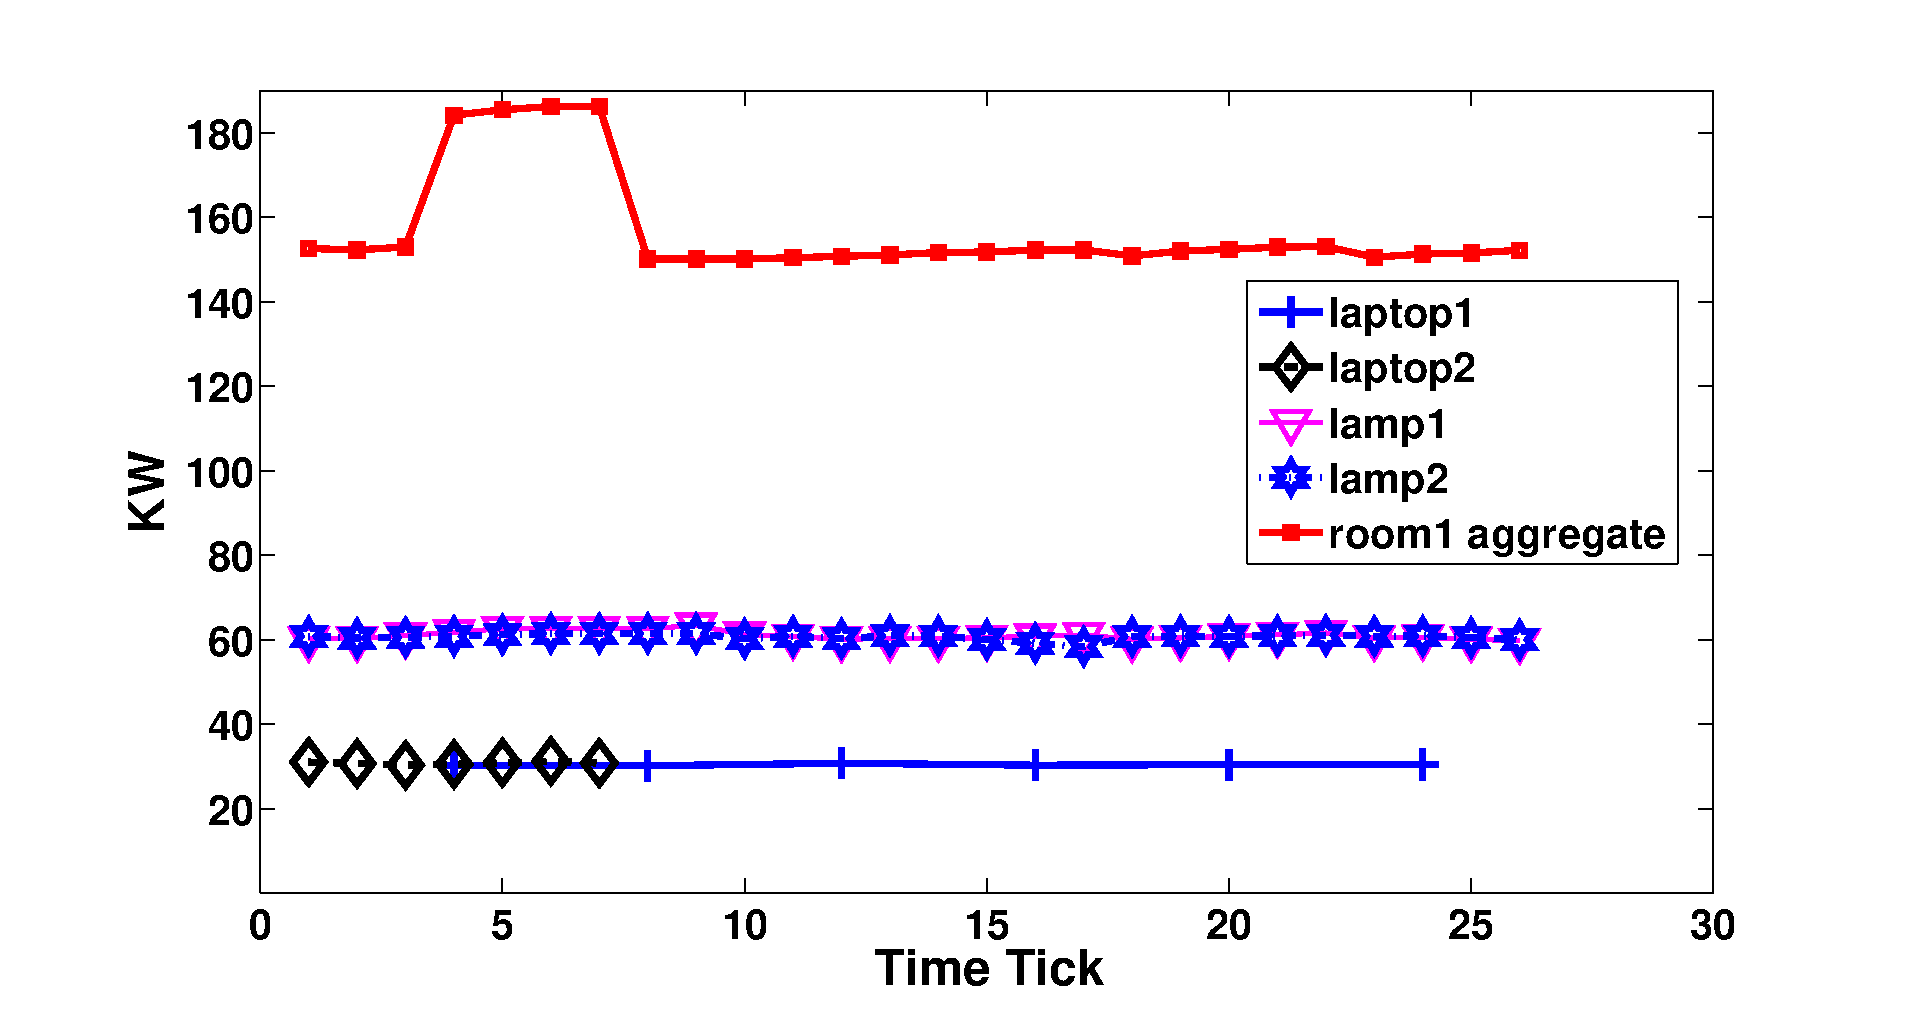
\includegraphics[scale=0.4]{figs/dynagg_scenario1_room1}
        }
\subfloat[Room 2 aggregate.]{%
            \label{fig:dynaggs1room2}
            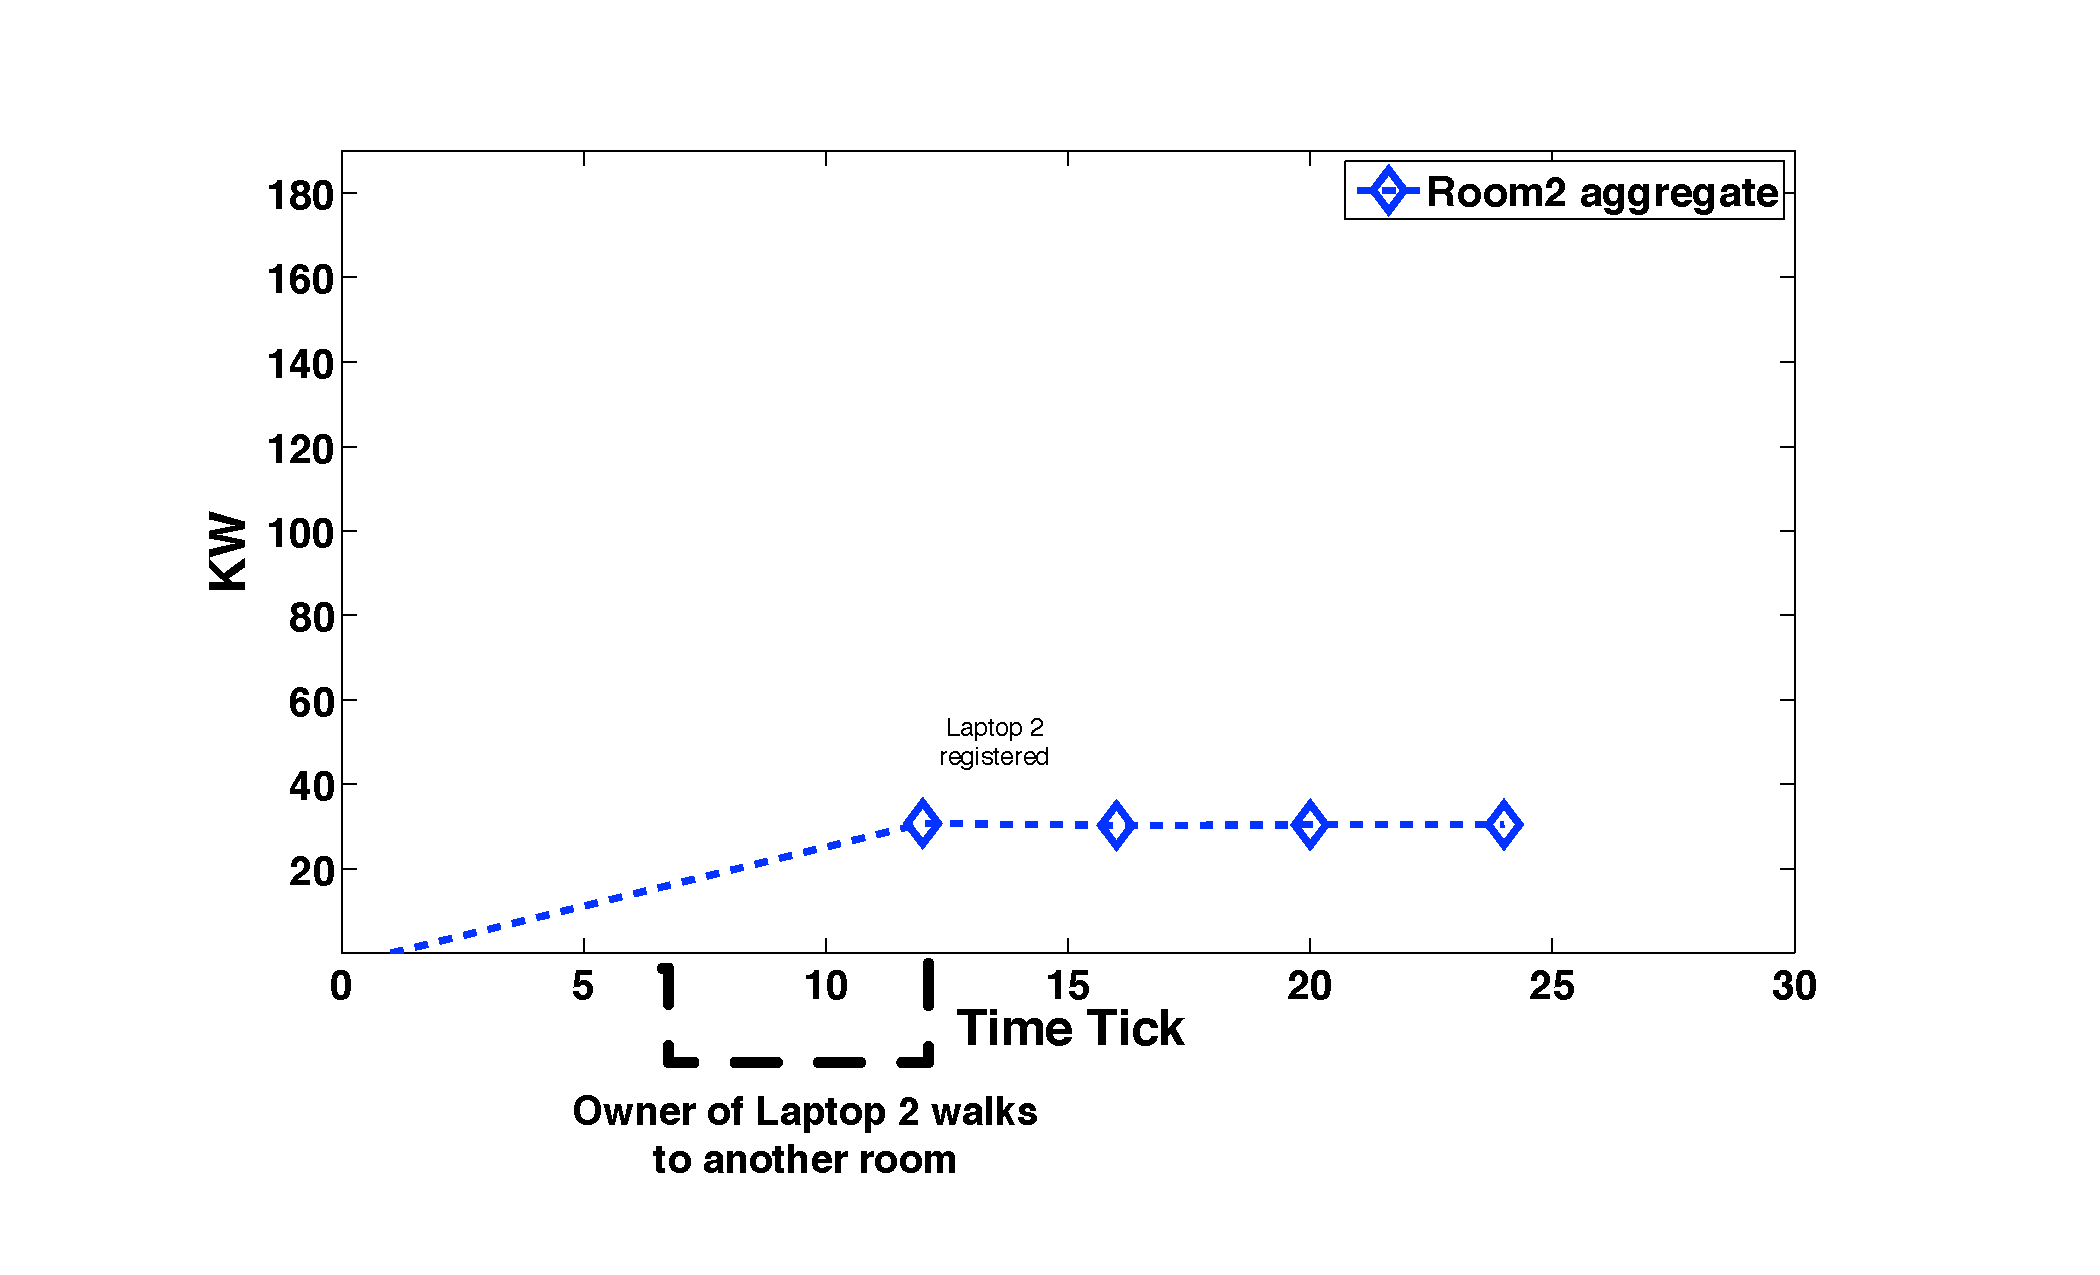
\includegraphics[scale=0.4]{figs/dynagg_scenario1_room2}
        }
\end{center}
\caption{
	The power consumes by a laptop in \emph{room 1} is shifted to \emph{room 2} a time t=7.  Notice the aggregagate drops in room 1
	while it rises in room 2.
     }%
\label{fig:multiroomagg}
\end{figure}

Figure~\ref{fig:multiroomagg} illustrate the aggregation results of that scenario.  Notice how...

% For demonstration lets have the user turn off on of their appliances when they leave as well.  This should cause that total
% room aggregate to drop, the person's personal aggregate to drop, but the other occupant's aggregate to remain
% the same.

% %FILL IN WITH REAL GRAPH
% \begin{figure}[htb!]
% \begin{center}
% 
\includegraphics[scale=0.39]{figs/blankbox}
% \caption{A room with items that belong to many users.  Person leaves with their item, aggregate falls.  Show aggregate.
% Person joins another room, aggregate in that room rises.  Show aggregate in the new room.  Compare before and after.}
% \label{fig:personaltotalagg}
% \end{center}
% \end{figure}

% Figure~\ref{fig:personaltotalagg} illustrate the results of the second sceanrio.  Note how...

%% \section{Experience Lessons learned}
% \begin{enumerate}
% \item engagement is necessary
% \item we must capture all devices, meters, \emph{and} their inter-relationship
% \item we must capture some location and other information about each entity for accounting
% \end{enumerate}

% \section{Challenges: Automation}
% \begin{enumerate}
% \item mobility
% \item bind-dissociation/re-association
% \item energy apportionment/accounting
% \end{enumerate}

\section{Projected results}
\begin{enumerate}
\item audit results
\item energy usage take-aways
\item query time for a typical single-device/lookup query
\item query time for an aggregate query
\end{enumerate}

% \begin{figure}[htb!]
% \begin{center}
% 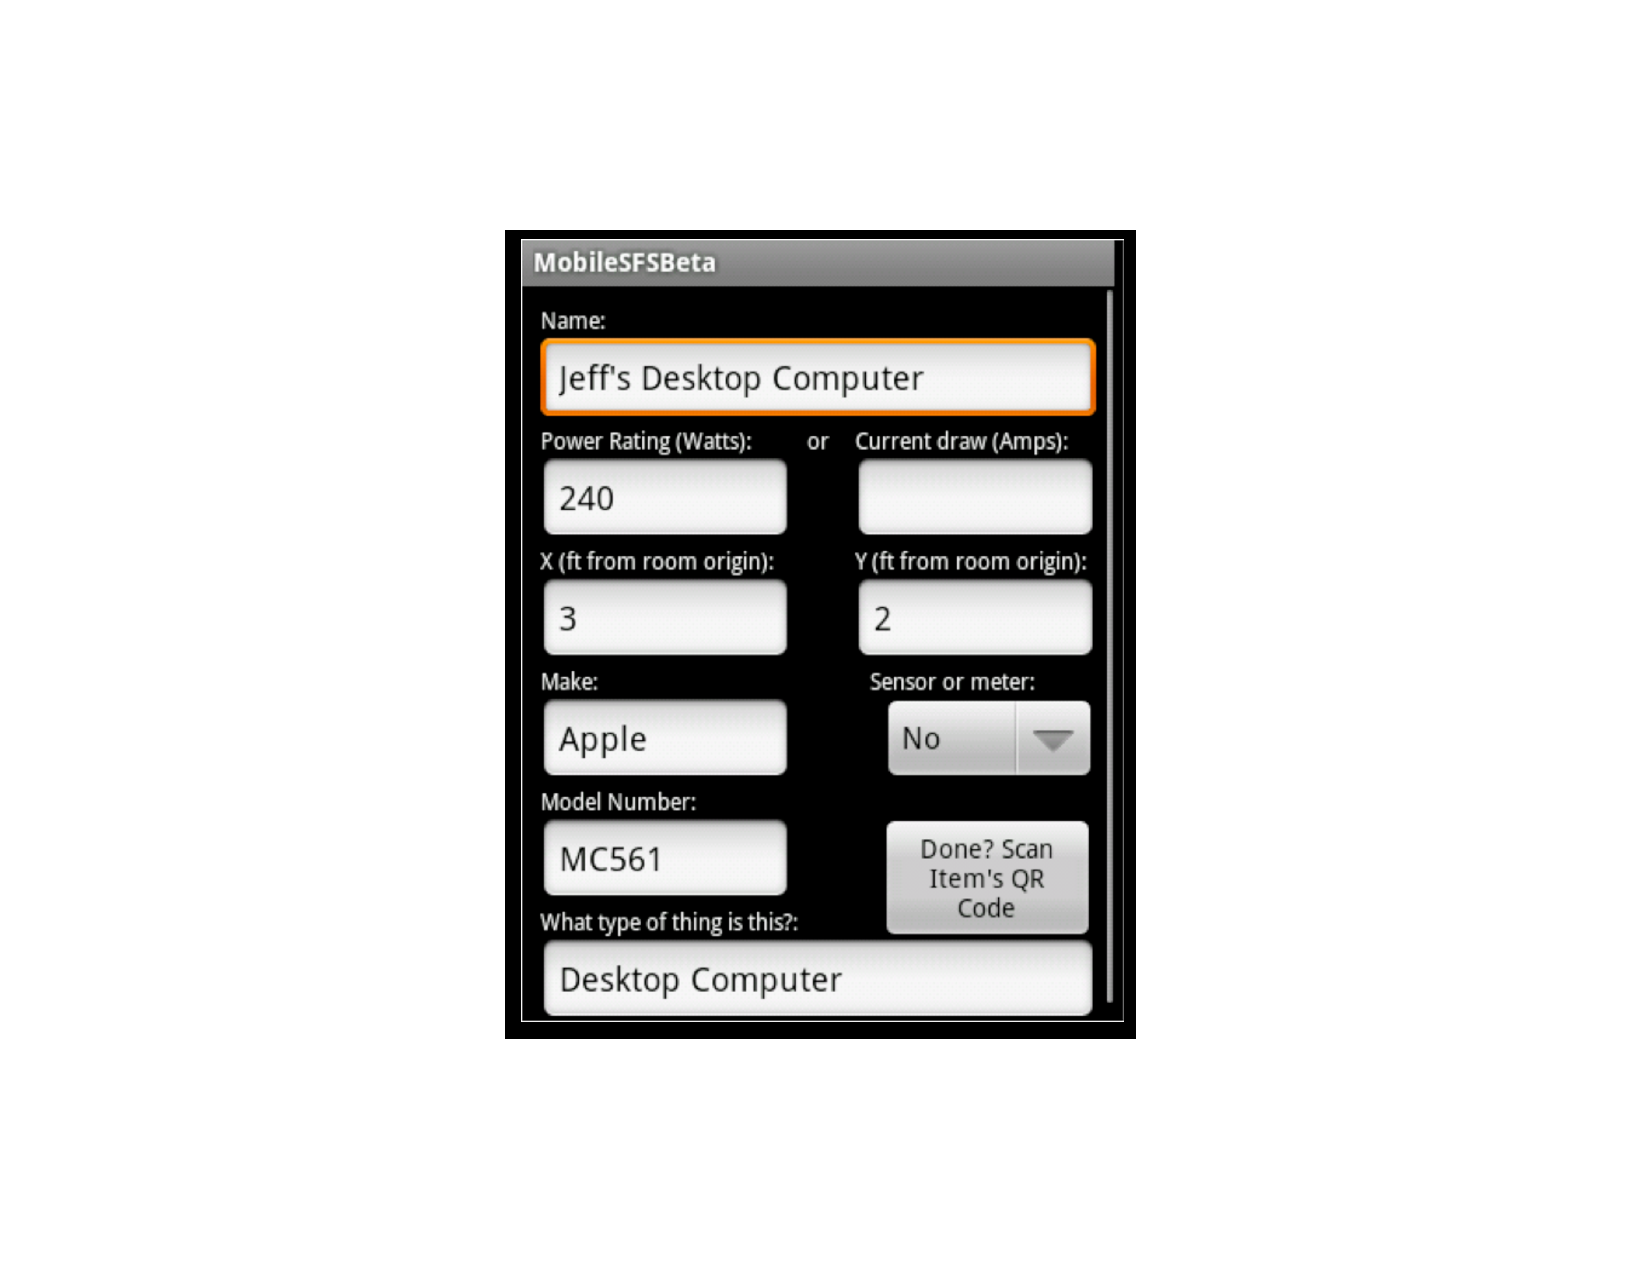
\includegraphics[width=0.8\columnwidth]{figs/screenshot01}
% \caption{The interface presented to the user for entering device and meter information.}
% \label{channelcomp}
% \end{center}
% \end{figure}



\section{Mobile SFS}
\label{sec:mobile}
The phone is the natural point of intersection between the user, the phyiscal world, and virtual services.\\

{\bf Goals}:
\begin{itemize}
\item Personalized energy attribution and tracking
\item Auto-aggregation techniques using stream correlation analysis \\
	\begin{itemize}
	\item identify stream correlations
	\item aggregate according to correlation threshold
	\item at user level, location level, total
	\item dealing with mobility (re-association and aggregation of streams) with dynamic subscriptions
	\end{itemize}
\end{itemize}

{\bf How do we know that the streams being aggregated are the right streams to aggregate?  What's the ground truth?}
Should we ask the user? (this becomes a user study)

The next approach skips this step altogether and establishes \emph{goodness} by comparing before/after aggregate consumption
data for the office.  Does the auto-aggregation help with this at all?

Is this about user engagement or is this about accuracy?  For a systems paper this really should be about accuracy
and should be compared against ground truth.  Ground-truth in this case is user behavior before and user behavior afterwards.


{\bf calibration might be an issue}

\begin{itemize}
\item Items that we were once used together that are no longer used together.
\item Energy consumption per user drops.
\item Cumulative energy consumption drops.
\end{itemize}

{\bf Accounts}:
\begin{itemize}
\item spaces
\item users \\
\end{itemize}

Users use their mobile phone to tag items they are actively using. \\

{\bf Tagging and registration mechanisms}:
\begin{itemize}
\item scan the qr code of the item you are currently using
\item if the item is a shared item, then it can be tagged by multiple users, and the energy can be split amongst all the users
	\begin{itemize}
	\item if a non-personal item is actively being used and nobody claims it, it is charged to all the users that we were in the same space
			as the item when the item became active.
	\item if a non-personal item is actively being used and nobody claims it and nobody was in the space when the item was turned on, it is charged
			to the space.
	\end{itemize}
\item if the item is a single-use item, it can only be used by a single user at time
\item if the item is a personal item, it can only belong to a single user and all energy is charged to that single user \\
\end{itemize}


{\bf Hypotheses}:

\begin{enumerate}
\item Personal energy attribution helps induce changes in behavior that lower energy consumption.
\item Personal energy attribution requires active user participation and engagement.
	\begin{itemize}
	\item Localization can be automated with indoor wifi; lowering participation overhead.
	\end{itemize}
\end{enumerate}



\subsection{Tracking steps}

\begin{enumerate}
\item Bootstrap
\item Tracking
\item Analysis
\item Visualization
\end{enumerate}


\subsubsection{Bootstrap}
The bootstrap phase is step where users become aware that there is energy information out there and it's the essential bootstrapping processes
of getting the user invovled in their energy attribution.  This step consists of:

\begin{enumerate}
\item Tagging items of everyday use with qr codes.
\item Binding meters and items.
\item Tag items as personal, shared, n-multi-shared
\end{enumerate}


All items should be tagged with qr codes.  This involves physically sticking a qr code onto the item, scanning it, and describing the item
that it is attached to.  This should be done for {\bf all items with a measurable energy footprint}, including lights, computers, appliances,
chargers, space heaters, etc.  -- miscenallenous eletrical loads.  A more advanced setup could include eletrical load information or HVAC 
component tagging, if visibility of total energy footprint is of interest.

Binding meters and items is a way of informing the system that the meter serves as an energy-consumption proxy for the item that the meter is
attached to.  This involves scanning both the meter and the item and creating their relationship explicitly.  This allows the application to query
the appropriate meter for historical consumption information when the user wishes to learn about the consumption of the item that is attached to that meter.
This model also assumes that meters are essentially free with respect to energy consumption.  Generally this assumption is not that far from reality.
For example, the ACme~\cite{acme} plugload meter draws on the order of several hundred milliwatts of power versus the tens to hundreds of watts being
consumed by the items it is typically measuring.

Tagging is the final, important step in the engagement phase.  This step requires that user scan items and essentially mark them as personal or shared.
This is used for analytical purposes and attribution.  You cannot determine which account the energy consumption of an item should be debited to without
ownership information.  Our application distinguishes between three types of sharing.  Personal items means that there is an owner relationship between
the item and its owner.  Any energy consumed by the item is attributed to the owner.  Shared items are charged to the user that last made use of the item.
If no user takes ownership of the item it is charged to every user of the system and each user is actively informed of the added charge (discussed in
section~\ref{sec:charge_alerts}).  Finally, the n-multi-shared items are items that can only be shared by N users at any one time.  This feature is essentially
sets an upperbound on the number of accounts that can be chared for the energy consumption of the device.

The cost of engagement is intially high but reduces over time.  The feature that we like best here is that the infrastructure captured through the engagement
step is beneficial for all users in the system and can be constructed iteratively.  The more users you have engaged, the faster the physical infrastructure
can be virtualized.

\subsubsection{Tracking}
%Scan you location/usage.

Tracking is the most active step in the attribution cycle.  This is where the user uses the application to record their location and energy consumption
information.  The infrastructure constructed in the \emph{bootstrap} step allows the user to scan their location and item being used.  For example, when the user walks into a building, she scans the qr code for the building to set their context.  As the user enters their office, they scan the qr code for the office.  Finally, 
before using any electrical device, the user scans it to register it's use.  Personal tags are most useful here, as they reduce this scanning step.
When the user is done using their item, they scan the item again to record that they are no longer using it.

This phase in the processes is the most tedious for the user and we think that more infrastructure and learning can be done to improve tracking.
To minimize interaction we offer mechanisms for grouping usage patterns.  For example, the user can decide to group items into an activity and 
combine streams for items that are associated with that activity.  For instance, each morning a graduate student comes to lab at the same time, 
turns on their PC or laptop, lamp, and prints out some papers.  The student pay group these streams into a single activity which alerts the application
to bin the energy consumed by the associated device to the account belonging to the user.

We also run correlation analysis in the background that looks to associate patterns of usage.  These may be presented to the user for corroboration
and ease the grouping processes.  We discuss its use in section~\ref{sec:correlation_analysis}.

% Analytical triggers

\subsubsection{Analysis}
Using traces generated by user activity, we track their energy usage through detailed accounting.  Our application combines energy consumption data
with contextual streaming data (i.e. location, usage information).  We perform aggregation in time, space, and category per user and group by activity
and location.  We also looks for trends in the data that indicate correlated usage patterns between items and users.  This allows us to ask
the user specific questions about grouping to make out analytics more accurate and reduce the burden imposed on the user during the tracking phase.
It also enables us to present the data to users about correlations amongst one another that could help them plan to use items more efficiently
from an energy perspective.  Details on our analysis is presented in~\ref{sec:analysis_results}.

\subsubsection{Visualization}
Finally, we looks for interesting ways of presenting real-time analytical data to users that could help them understand their own energy usage, as
well as the context of energy usage in their environment.  Our specific aim in this phase is to induce changes in behavior that cause the user to
make better use of their devices and reduce their overall energy consumption.  We demonstrate some of the visualization in section~\ref{sec:viz}
and the overall energy consumption before and after using the application in section~\ref{sec:energy_before_after}.


\section{Results}
This section will go start, first by talking about the overall energy consumption results.  For this, a baseline must be established, either
at the room-aggregate level or the individual user level.  The latter is simpler and is useful for comparing the effect of the system on invidual
energy consumption.  That's really the point of the system.






\subsection{Limitations}
EMD is useful for finding underlying behavioral relationships between traces of sensor data.  However,
when we set the timescales smaller than a day, the results were not as strong.
The trace has to be long enough to capture the trend.  For this data set, the underlying
trend is daily, therefore it requires there to be a significant number of samples over many days.
%  to
% for this method to be effective.
Although this was a limitation for this dataset, it really depends on the underlying phenomenon that
the sensors are measuring.  Its underlying trend is ultimately what EMD will be able to separate
from the intrinsic modes of the underlying signal.

\subsection{Discussion}
EMD allows us to effectively identify fundamental relationships between sensor traces.
% Using EMD to find fundamental relationships between sensor traces effectively identifies intrinsically
% related behavioral relationships.
% was quite promising for building
% up models of correlated usage.  
We believe that identifying meaningful usage-correlation patterns can help reduce oversights
by the occupants and faults that lead to energy waste.  A direct application of this is the identification
of simultaneous heating and cooling~\cite{simheatcool}.  Simultaneous heating and cooling is when heating
and cooling system either compete with one another or compete with the incoming air from outside and is
a cause for major energy waste in building~\cite{simheatcool}.  The longer it goes undetected,
the more waste there is.  However, it is very difficult to identify since the occupants do not notice
changes in temperature.  Our analysis can be used to build a correlation model between the outside
heating cooling temperature, the cooling coil temperature, and the outside air vent position.  If their behavior
is not correlated as expect, an alarm should be raised.

We can also apply it to other usage scenarios.  In our traces, for example, we found an instance where the pump
was on, but the lights were off.  The two are typically correlated, however, in this case they were not.
The air conditioning was pumping cool air into a room without occupants.
With our approach this could have been identified and corrected.  In future work, we intend to
package our solution to serve these kinds of applications.

% EMD works perfectly although the weekly pattern of the data is altered the last analyzed week.

% EMD inherently finds the interesting time scales.

% number of zero crossing = mean frequency/time scale:
%   TODO give the time scale for each IMF.


\section{Conclusion}
% what is our problem

% what we did

% contributions and main results

% future work


This paper set out to examine the underlying relationship between sensor traces to find interesting correlations
in use.  We used data from a large deployment of sensors in a building and found that direct correlation analysis on the raw
traces was not discriminatory enough to find interesting relationships.  Upon closer inspection, we noticed that
the underlying trend was dominating the correlation calculation.  In order to extract meaningful behavior this trend has
to be removed.  We concluded that empirical mode decomposition is a helpful analytical tool for de-trending 
non-linear, non-stationary data; inherent attributes contained by our traces.

We re-ran our analysis on the same traces, except we correlated the IMF outputs of the EMD operation on each of the traces and found that the pump was closely related to the lights in the same room served by the pump and
uncorrelated with a pump on the same floor serving a different room.  In order to corroborate the applicability
of our approach, we compared the pump trace with \emph{all} 674 sensor traces and found a strong correlation
between the relative spatial position of the sensors and their IMF correlations.  The most correlated IMFs were 
serving the same
area in the building.  As we relax the admittance criteria we find that the spatial correlation expands radially from
the main location served by the reference trace.

We plan to examine the use of this method in applications that help discovery changes in underlying relationships over time
in order to identify opportunities for savings in buildings.  We will use it to build inter-device correlation models
and use these models to establish ``normal'', ``abnormal'' usage patterns.  We hope to take it a step further and include a
supervised learning approach to distinguish between ``efficient'' and ``inefficient'' usage patterns as well.








\vspace{+0.5mm}
\vspace{+2mm}
\bibliographystyle{abbrv}
%\scriptsize
\bibliography{references}
%\bibliography{references}

\end{document}


